\documentclass[output=paper]{langscibook}
\ChapterDOI{10.5281/zenodo.8124494}
\author{Eduardo Tadeu Roque Amaral\affiliation{Universidade Federal de Minas Gerais} and Wiltrud Mihatsch\orcid{}\affiliation{Universität Tübingen}}
\title{Portuguese \textit{a pessoa} and \textit{uma pessoa}: Emerging inclusive impersonals}
\abstract{In both Brazilian and European Portuguese, \textit{a pessoa} (‘the person’), \textit{uma pessoa} (‘a person’), \textit{as pessoas} (‘the persons’), \textit{o povo} (‘the people’), \textit{o pessoal} (‘the people’) and some other, more colloquial expressions such as \textit{geral} ‘general’ \parencitetv{chapters/07-Avelar} are currently developing new impersonal uses (see \citealt{Afonso2008}, \citealt{AmaralMihatsch2019}, \citealt{Posio2021}). In this contribution we will analyse the functional changes of \textit{a pessoa} and \textit{uma pessoa}, with a focus on Brazilian Portuguese. Interestingly, all these expressions are originally third person noun phrases excluding reference to speakers and addressees. In impersonal contexts, however, \textit{a pessoa} and \textit{uma pessoa} are predominantly used in non-referential contexts where speaker and addressee may be included. We will try to shed light on the evolution of the functions of the emerging impersonal pronouns \textit{a pessoa} and \textit{uma pessoa} in Brazilian Portuguese, starting with a macro-diachronic analysis tracing the earliest impersonal uses on the basis of the Corpus do português (CDP, Genre/Historical) by Mark Davies and by comparing Brazilian oral colloquial data from the 20th century based on the comparative subcorpus of NURC RJ with contemporary corpus data from Rio de Janeiro (CORPORAPORT) and Minas Gerais (MOC). The corpus analysis will be complemented by acceptability judgments. The different data types will be combined in order to trace the diachronic development of the restrictions determining the impersonal uses and the differences and parallels between the two expressions. We will close by comparing our results with existing studies by \citet{Posio2017, Posio2021} and \citet{Martins2022} on parallel developments in European Portuguese.}
\IfFileExists{../localcommands.tex}{
  \addbibresource{../localbibliography.bib}
  \usepackage{langsci-optional}
\usepackage{langsci-gb4e}
\usepackage{langsci-lgr}

\usepackage{listings}
\lstset{basicstyle=\ttfamily,tabsize=2,breaklines=true}

%added by author
% \usepackage{tipa}
\usepackage{multirow}
\graphicspath{{figures/}}
\usepackage{langsci-branding}

  
\newcommand{\sent}{\enumsentence}
\newcommand{\sents}{\eenumsentence}
\let\citeasnoun\citet

\renewcommand{\lsCoverTitleFont}[1]{\sffamily\addfontfeatures{Scale=MatchUppercase}\fontsize{44pt}{16mm}\selectfont #1}
   
  %% hyphenation points for line breaks
%% Normally, automatic hyphenation in LaTeX is very good
%% If a word is mis-hyphenated, add it to this file
%%
%% add information to TeX file before \begin{document} with:
%% %% hyphenation points for line breaks
%% Normally, automatic hyphenation in LaTeX is very good
%% If a word is mis-hyphenated, add it to this file
%%
%% add information to TeX file before \begin{document} with:
%% %% hyphenation points for line breaks
%% Normally, automatic hyphenation in LaTeX is very good
%% If a word is mis-hyphenated, add it to this file
%%
%% add information to TeX file before \begin{document} with:
%% \include{localhyphenation}
\hyphenation{
affri-ca-te
affri-ca-tes
an-no-tated
com-ple-ments
com-po-si-tio-na-li-ty
non-com-po-si-tio-na-li-ty
Gon-zá-lez
out-side
Ri-chárd
se-man-tics
STREU-SLE
Tie-de-mann
}
\hyphenation{
affri-ca-te
affri-ca-tes
an-no-tated
com-ple-ments
com-po-si-tio-na-li-ty
non-com-po-si-tio-na-li-ty
Gon-zá-lez
out-side
Ri-chárd
se-man-tics
STREU-SLE
Tie-de-mann
}
\hyphenation{
affri-ca-te
affri-ca-tes
an-no-tated
com-ple-ments
com-po-si-tio-na-li-ty
non-com-po-si-tio-na-li-ty
Gon-zá-lez
out-side
Ri-chárd
se-man-tics
STREU-SLE
Tie-de-mann
} 
  \togglepaper[5]%%chapternumber
}{}
\begin{document}
\maketitle

\section{Introduction}

A considerable number of studies have shown the existence of impersonal and personal pronouns that originate from noun phrases with highly general human nouns such as French {\textit{on}} {(impersonal ‘one’ or ‘you’) or Portuguese} {\textit{a gente}} {(personal pronoun ‘we’ with an earlier impersonal meaning, from} {\textit{a gente}} {‘the people’). In Brazilian Portuguese (BP) and European Portuguese (EP) there are several expressions such as} {\textit{a pessoa}},{ \textit{uma pessoa}},{ \textit{as pessoas}},{ \textit{o povo} }{and}{ \textit{o pessoal}} {which take over impersonal functions (\citealt{AmaralMihatsch2019, Posio2021}). However, although all these expressions are originally third person noun phrases excluding speakers and addressees,} {\textit{a pessoa}} {(literally ‘the person’) and} {\textit{uma pessoa} }{(literally ‘a person’) are particularly used in contexts where speaker and addressee are included. This study aims to analyse these expressions in order to shed light on the different restrictions determining the exclusive and inclusive impersonal uses and their referential functions, starting out with the classification by \citet{GastvanderAuwera2013}. As typically observed in other processes of grammaticalisation, the functional changes are accompanied by other, rather formal changes not focused on in this study (but see \citealt{Posio2021} for European Portuguese and \citealt{AmaralMihatsch2019} for Brazilian Portuguese), such as their increasingly common occurrence in the syntactic subject position, decategorialisation, which leads to the loss of gender and number inflection and the possibility of adjectival modification, a certain degree of prosodic weakening \citep{Posio2021} and more specific developments leading to well-established impersonal pronouns such as the impossibility of referring anaphorically to an impersonal antecedent (\citealt{CabredoHofherr2008}: 39--42, 45--48).}



{\citet{Posio2021} analyses these constructions in EP and discusses their status as potentially grammaticalised referential devices. \citet[3]{Posio2021} assumes that human impersonal referential devices, in opposition to prototypical personal pronouns (such as} {\textit{I}} {or} {\textit{you}}{), receive their interpretation through inference rather than reference. In example \REF{ex:amaral:1}, according to \citet[11]{Posio2021}, the NP} {\textit{a}} {\textit{pessoa} }{‘the person’}{ }{gains its speaker-oriented interpretation by inference from the immediate discourse context. The statement about the speaker’s life and work, formulated in the first person plural, is followed by the generalising but still inclusive expression} {\textit{a pessoa}}{, corresponding to English} {\textit{one.}} {This is another typical use of the} {\textit{pessoa}} {constructions, as will be confirmed by our analysis.}


\ea\label{ex:amaral:1} 
 penso que o trabalho absorve-nos muito, (1.3) e acho que nos ocupa mesmo muito atualmente
 \glt ‘I think that the work absorbs us a lot, (1.3) and I think that it occupies us really a lot these days’\\
 acho que {\ExHighlight{a pessoa}} vive muito para o trabalho. (.) e já sai do trabalho muito cansada. (0.6) {eh:}{(0.4)}
 \glt ‘I think that \ExHighlight{the person} lives a lot for the work. (.) and already leaves the job really tired. (0.6) eh: (0.4) \citep[11]{Posio2021}
\z 
    

{Based on previous studies, \citet{Posio2017,Posio2021} points out some differences between EP, BP and Peninsular Spanish varieties in the domain of human impersonal constructions. Although Spanish is a language syntactically close to Portuguese, it does not present evidence of a grammaticalisation process resembling the} {\textit{pessoa} }{constructions, but both EP and BP do, and recent research has shown some interesting similarities and differences between them. \citet{Posio2021} highlights that it is not surprising that a construction resembling the} \textsc{man}-im\-per\-son\-als has emerged in the varieties of Portuguese but not in Spanish, since Brazilian Portuguese and to some extent European Portuguese \citep[346]{Posio2012} do now fill the subject position more frequently and in more contexts than Spanish (see the chapters in \citealt{KatoNegrão2000} and \citealt{LamogliaDuarte2000}). The impersonal uses of {\textit{a pessoa}} {and} {\textit{uma pessoa} }{are thus a particular feature of Portuguese within the Ibero-Romance language family. When translating the above example into Spanish, the use of the non-grammaticalised Spanish NPs} {\textit{la persona}} {and} {\textit{una persona}} leads to the loss of the impersonal reading and in many cases the use of this etymological equivalent sounds awkward. This is clear evidence of functional changes occurring beyond contextual effects and mere inference, by which these expressions have changed. 



{This contribution focuses on the diachronic and, to some extent, diatopic tendencies in the referential functions of these emerging impersonals. Our analysis is structured as follows: the next section (\sectref{sec:amaral:2}) will give an overview of the main functions and properties of impersonal pronouns. In \sectref{sec:amaral:3} we will sketch the known paths of pronominalisation of impersonal pronouns and formulate a hypothesis as to how} {\textit{a pessoa} }{and} {\textit{uma pessoa}} {might have emerged and the degree to which their paths might be related. The following section \sectref{sec:amaral:4} will explain the methodology. In \sectref{sec:amaral:5}, we present our diachronic corpus analysis, starting with the earliest uses in the} {\textit{Corpus do Português}} (CDP) {Genre/Historical and ending with 21st{}-century colloquial data from Brazil. We will bring together the results of the corpus analysis in \sectref{sec:amaral:6}, where we will outline the most important referential changes of} {\textit{a pessoa}} {and} {\textit{uma pessoa}} {and point out parallels and differences between BP and EP. These results will be complemented by some of our results from a large-scale acceptability study before we close with a brief conclusion.} 



\section{Impersonality and impersonal pronouns}\label{sec:amaral:2}



{There are various discourse contexts or communicative settings where speakers need or want to avoid specifying arguments that must be expressed syntactically, for instance when speakers make general} {statements, when they want to avoid naming known referents or when they ignore the identity of referents. This is particularly important for the subject position, which is typically occupied by an argument referring to a human agent. This position needs to be filled in non{}-pro-drop languages such as French and is increasingly filled in Brazilian Portuguese (see, for instance, \citealt{Kato2000}). In European Portuguese it may also be filled even when subject expression is not syntactically, semantically or pragmatically obligatory \citep[346]{Posio2012}. This is also one reason, at least for non-pro-drop languages, why many impersonal pronouns occur in the subject position, as in the case of French} {\textit{on}}{, or at least prefer the subject position as in the case of English} \textit{one}. Similarly, in the pro-drop language Spanish the impersonal pronoun \textit{uno} ‘one’ occurs most often although not exclusively in the subject position \parencites[43--44]{CabredoHofherr2008}[263]{CabredoHofherr2017}. Other aspects play a role in explaining the preference for the subject position, for instance the correlation between the subject position and agency and the frequency of subjects referring to humans.



Apart from the above-mentioned speaker motivations, impersonal pronouns thus allow the subject position to be filled without specifying the referents, a function captured by the definition offered by  \citet[124]{GastvanderAuwera2013}:



\begin{quote} Impersonalization is the process of filling an argument position of a predicate with a variable ranging over sets of human participants without establishing a referential link to any entity from the universe of discourse.\\\hbox{}\hfill\hbox{(\citealt[124]{GastvanderAuwera2013})}\end{quote}



The crucial difference between impersonals and other pronouns is indeed their lack of referential anchoring, i.e. they do not introduce new discourse referents that can be taken up anaphorically (see \citealt{Siewierska2011}: 67), which is a consequence of their primary function, agent defocusing \citep[52--55]{Achard2015}.



Impersonal pronouns, i.e. different types of fillers of argument positions, go back to several distinct types of diachronic sources. They may go back to lexical sources, in most cases general human nouns meaning ‘human being’ as in the case of the so-called \textsc{man}-impersonals such as French \textit{on} or German \textit{man}, but also collective or plural general human nouns with the meaning ‘people’, as in the case of the earlier impersonal uses of Portuguese \textit{a gente} and the incipient impersonal uses of Portuguese \textit{as pessoas}, \textit{geral}, \textit{(a) galera},  \textit{(o) povo}, \textit{(o) pessoal} (\citealt{AmaralMihatsch2019, SilvaCoelho2020}, \citetv{chapters/07-Avelar}); a similar tendency has been observed for French \textit{les gens} (\citealt{CappeauSchnedecker2015}). 



Another important source for impersonal pronouns are personal pronouns as in the case of the impersonal uses of second person pronouns (see \citealt{Kluge2016}) and third person plural pronouns \citep{Siewierska2011}, but also indefinite pronouns as in the case of English {\textit{one}} \citep{Moltmann2010} or Spanish \textit{uno} (\citealt{CompanyPozas2009}). Notably, we thus find both definite and indefinite sources.



The evolution of the impersonal pair \textit{a pessoa/uma pessoa} with both a definite and an indefinite source is still unclear and we do not know for sure whether they have a common source or two separate sources. Related to their diachrony, we need to find out whether they are functionally equivalent, and whether there are any differences between BP and EP.



\section{The evolution of impersonal pronouns and the case of \textit{a pessoa/uma pessoa}}\label{sec:amaral:3}



{\textit{A pessoa} }{and} {\textit{uma pessoa} }{share their function of agent defocusing and their emerging status as pronouns, as suggested by \citet{AmaralMihatsch2019} and \citet{Mihatsch2017}. The more established impersonal pronouns (e.g. French} {\textit{on}}{, Portuguese} {\textit{a gente}}{) are known to go back to different sources:  a generic NP in the case of} {\textit{on}}{ (see  \citealt{GiacaloneRamatSansò2007, GiacaloneRamatSansò2011}), and a definite referring NP with plural reference as in the case of} {\textit{a gente}} {‘the people’ (see \citealt{Lopes2003,Lopes2004}) or in the emerging impersonals} {\textit{as pessoas}} {‘the persons’ and} {\textit{o povo} }{‘the people’. The sources are linked to particular discourse strategies, which also explains some of their contemporary functional differences (\citealt{AmaralMihatsch2019}). We will start out with Gast \& van der Auwera’s semantic map}\footnote{Semantic maps visualise synchronic relations between functions typically expressed by polysemous items as well as diachronic relations (see \citealt{Haspelmath2003}). Neighbouring functions on a semantic map typically show minor differences.} {of impersonal pronouns, refining some aspects. The circular map established by \citet{GastvanderAuwera2013} for impersonal pronouns synthesises the functions distinguished for the well-studied} {\textsc{man}}{{}-impersonals and impersonals based on third person plural pronouns (see \citealt{Siewierska2011} and \citealt{CabredoHofherr2006,CabredoHofherr2008}, and others). \citet{GastvanderAuwera2013} distinguish seven main functional clusters, which are each related with the preceding and following cluster, with a link between functions 1 and 7 closing the circle. In what follows we will adopt their terminology: S refers to the sentence type and HP to the properties of the human participants (\citealt{GastvanderAuwera2013}: 27). Sentence contexts can be either veridical or non-veridical, i.e. not showing truth values, as is the case with conditionals or questions and generally modal contexts such as hypothetical sentences. Episodic sentences are anchored in time and space and refer to particular (but not necessarily identifiable) referents, whereas generic sentences are not anchored in any specific point in time or specify any particular referents. Furthermore, impersonals can include or exclude the speaker or, if the speaker is not included, can be oriented toward the speaker and adopt the perspective of the speaker.}

\tabref{tab:amaral:1} summarises and illustrates this classification.


\begin{table}
    \begin{tabular}{ll}
    \lsptoprule
    {1.} & {S: veridical/episodic, HP: existential/indefinite/vague}\\
    & {\textit{They’re knocking on the door.}}\\ 
    \midrule
    {2.} & {S: veridical/episodic, HP: existential/indefinite/plural}\\
    & {\textit{They’ve surrounded us.}}\\
    \midrule
    {3.} & {S: veridical/episodic, HP: existential/definite}\\
    & {\textit{They’ve raised the taxes again.}}\\
    \midrule
    {4.} & {S: veridical/generic, HP: universal, external}\\
    & {\textit{They eat dragonflies in Bali.}}\\
    \midrule
    {5.} & {S: veridical/generic, HP: universal, internal}\\
    & {\textit{One only lives once}}.\\
    \midrule
    {6.} & {S: non-veridical/modal, HP: universal, internal}\\
    & {\textit{One should never give up.}}\\
    \midrule
    {7.} & {S: non-veridical/non-modal, HP: universal, internal}\\
    & {\textit{What happens if one drinks sour milk?}}\\
    \lspbottomrule
    \end{tabular}
    \caption{Clusters of properties of impersonal pronouns (\citealt{GastvanderAuwera2013}: 27)}
    \label{tab:amaral:1}
\end{table}





The distinctions between inclusive and exclusive, episodic and generic and veridical or non-veridical uses seem to be binary ones. However, there are degrees of inclusiveness, ranging from a clear reference including the speaker to differing degrees of speaker orientation, or degrees of episodicity with more or less explicit and specific temporal anchors, or degrees of universality, between the reference to a totality (humankind in 5) to vague spatio-temporal restrictions as in function 4 in \tabref{tab:amaral:1}. 



{The link between function 1 and function 7, leading to a circular map, might not be obvious at first sight. When we take into account the closeness and referential equivalence of the indefinite pronouns} {\textit{someone}} {or} {\textit{somebody}} {and the impersonals in these contexts, this link becomes plausible. The contrast between functions 1 and 7 regarding inclusiveness is a pragmatic effect which  \citet[154]{GastvanderAuwera2013} relate to informativity in discourse, with a highly marked and therefore unlikely inclusive interpretation for episodic contexts as in function 1. Nevertheless, impersonal pronouns may also develop inclusive episodic readings, and they may leave the domain of impersonals and become first person personal pronouns as in the cases of BP} {\textit{a gente}} {\citep{Lopes2004} or French} {\textit{on}}{. In what follows we will situate known grammaticalisation paths of impersonal pronouns with respect to these functions, point out the main differences between the grammaticalised uses and the non-grammaticalised source constructions and try to position the evolution of} {\textit{a pessoa} }{and} {\textit{uma pessoa}} {with respect to the semantic map and the known paths.}



{The most detailed diachronic analyses exist for} {\textsc{man}}{{}-impersonals, which are considered an SAE feature}\footnote{The linguistic area of Standard Average European (SAE) covers Romance, Germanic, Balto-Slavic, Balkan and to some extent Finno-Ugrian, which share a number of grammatical features due to contacts in late antiquity (\citealt{Haspelmath2001}).} {well{}-attested in many European languages, including Ibero-Romance languages, at least in the medieval period (\citealt{GiacaloneRamatSansò2007}). They only survive in some languages such as French} {\textit{on}} {and German} {\textit{man}} {and Mainland Scandinavian \citep{Egerland2003}, while they disappeared from Portuguese and Spanish in the 16th century (\citealt{CompanyPozas2009}, \citealt{Lopes2003}: 54). The source construction is a generic noun phrase with a lexical noun ‘man, human being’. Generic NPs are, of course, not restricted to humans although, in the case of generic NPs with general human nouns, we automatically arrive at a speaker-inclusive interpretation. It is crucial for the study of these pronominalisation processes to consider NPs and not just lexical items. This is easily overlooked since} {\textsc{man}}{{}-impersonals do not show any determiners. The starting point of the process of pronominalisation is the medieval or even earlier singular generic bare NP, at a time when the generic function of the definite article is gradually developing (a process fossilised in the French impersonal variant} \textit{l’on}). It is notable that the indefinite article cross-linguistically develops its generic readings rather late, in the 16th century in Romance languages, and is generally the last step in the evolution of indefinite articles as in the case of Spanish {\textit{un(a)}} {‘a’ (see \citealt{Givón1978,Givón1981}, \citealt{Elvira1994}: 48).}



{In the analysis of} {\textsc{man}}{{}-impersonals, the generic reading as illustrated in the following example does not require grammaticalisation:}
\ea\label{ex:amaral:2}
 Non in solo pane vivit \ExHighlight{homo} {(Matthew 4:4)\\
 \glt‘Man does not live by bread alone’ (\citealt{GiacaloneRamatSansò2007}: 100)}\\
\z 


Generic uses as a source of impersonals are associated with particular discourse traditions. \citet[1171--1174]{CompanyPozas2009} identify the role played by religious and moral genres for this development in Old Spanish. In these texts the positing of general truths about human beings is highly relevant. The kind-reference is lost as the impersonal use arises. This is evident in the Old Italian example in \REF{ex:amaral:3}, a hypothetical context corresponding to function 7 in \tabref{tab:amaral:1}, the point where \textsc{man}-impersonals enter the domain of impersonals:

\ea\label{ex:amaral:3}
 ...quando \ExHighlight{{uomo}} truova la donnola nella via… (Novellino, 32, rr. 7--8)\\
 \glt ‘When one finds a weasel on his [sic] way’ (\citealt{GiacaloneRamatSansò2007}: 101)\\
\z 

Here, {\textit{uomo}} {refers to any member of humanity but not to humankind, and it is referentially equivalent to the indefinite pronoun} {\textit{one}} {(see also \citealt{GiacaloneRamatSansò2011}: 94). In the course of grammaticalisation these impersonals may subsequently adopt the other functions from 6 to 1 in \tabref{tab:amaral:1}. An indicator for the generic source are the first uses in non-episodic non-referring contexts and the still prevailing generic or non-episodic inclusive use of the less entrenched} {\textsc{man}}{{}-impersonals in peripheral areas of the SAE languages (\citealt{GiacaloneRamatSansò2007}).}



{Well-entrenched impersonals (such as English} {\textit{one}}{, going back to a different source, however) can be distinguished from generic uses of general human nouns. Our English example \REF{ex:amaral:4} features a fossilised bare generic use of} {\textit{man}}{, which can also be capitalised (OED, s.v.} {\textit{man}}{), while the pronoun} {\textit{one}} {cannot refer to the kind and therefore cannot replace} {\textit{man}} {in this use:}

\ea\label{ex:amaral:4}
With the agricultural revolution, \ExHighlight{man} started to settle down, but still many followed a wandering path throughout history.\\ (\url{https://eu.coloradoan.com/story/opinion/2017/07/07/editorial-fort-collins-should-stay-course-homeless-services/449108001/}{, page last consulted on 28/04/2022)}
\z 


The referentially equivalent lexical item as well the definite article of \textit{a pessoa} might suggest an analogous path of pronominalisation. In order to clarify this question we need to look at different types of generic NPs. 



In English, as well as in other modern European languages with a strongly grammaticalised definite and indefinite article, there are two basic ways of establishing generic reference (see \citealt{KrifkaGerstner-Link1993}, \citealt{Krifka1995}). The definite article (singular and plural) may directly refer to kinds. This is why they are common with kind predicates, shown in the Portuguese examples taken from \citet{BarraFerreiraNunesCorreia2016}:

\ea\label{ex:amaral:5}O urso polar está quase extinto. {(BP, EP)}
\glt ‘The polar bear is almost extinct.’
\ex\label{ex:amaral:6}Os ursos polares estão quase extintos. {(BP, EP)}
\glt ‘The polar bears are almost extinct.’
\z 

Kind-generic uses also allow plural (and singular) interpretations: 

\ea\label{ex:amaral:7}The antelope gathers near waterholes. (\citealt{KrifkaGerstner-Link1993})\z 

\begin{sloppypar}
We believe that this flexibility eases the subsequent step of grammaticalisation of {\textsc{man}}{{}-impersonals. Relevant for the grammaticalisation processes of impersonal pronouns is the distinction between the previously described kind-generic interpretation (D-genericity according to \citealt{KrifkaGerstner-Link1993}) and generic readings with the indefinite singular article. According to \citet{KrifkaGerstner-Link1993} this is a case of I-genericity arising at the sentence level. We suggest that diachronically, indefinite articles must have undergone changes to allow for these uses which, as mentioned above, arise relatively late. \citet{KrifkaGerstner-Link1993} argue that indefinite generic uses are tied to modal uses and habitual uses. We think that diachronically the generic uses of indefinite NPs arise from the communicative strategy of exemplification, i.e. generalisations based on selecting one exemplar that represents the kind. This also explains why indefinite generics cannot refer to accidental properties such as} {\textit{popular} }{as in \REF{ex:amaral:8} and \REF{ex:amaral:9}, since this property does not necessarily apply to each exemplar but, rather, is a typical feature characterising many instances of the whole category. Although the property} \textit{popular} does not apply to each instance, it is a characteristic feature of the whole kind, therefore allowing the definite generic NP, which does not show this restriction:
\end{sloppypar}

\ea[]{\label{ex:amaral:8}The madrigal is popular. / The madrigal is polyphonic.}
\ex[*]{\label{ex:amaral:9}A madrigal is popular. / A madrigal is polyphonic. (\citealt{KrifkaGerstner-Link1993})}
\z 


We think that the exemplar-based generalisation not requiring an established category (but an applicability of a predicate to each instance) also explains the flexible noun selection of sentences with indefinite generics as opposed to the restriction of definite generics to well-established kinds (\citealt{KrifkaGerstner-Link1993}). There is no well-established category ‘green bottle’, therefore the definite generic NP is not possible (example~\ref{ex:amaral:10}). However, the generalisation starting out from one exemplar is a cognitive strategy for allowing new categories to be created (see \citealt{Barsalou1983} and \citealt{Mauri2017} on the linguistic means of creating ad hoc categories) and since the indefinite generic is based on a generalisation strategy starting out from a representative instance, its use is not restricted to well-established categories, but can also refer to ad hoc categories such as \textit{green bottle}:

\ea[*]{\label{ex:amaral:10}The green bottle has a narrow neck.}
\ex[]{\label{ex:amaral:11}A green bottle has a narrow neck.}
\z 


{As for the evolution of} {\textsc{man}}{{}-impersonals, the early contexts of use in moral and religious texts (\citealt{GiacaloneRamatSansò2007}) go far beyond focusing on just the essential properties of the human species applying to each individual. At the same time the human species is a well-established kind. Therefore definite generics must be the source of} {\textsc{man}}-impersonals, although the medieval bare NPs do not give us a direct formal clue.



{Could} {\textit{a pessoa} }{also arise in definite generic contexts? Our own previous lexical analyses of French, Spanish and Portuguese cognates of PERSŌNA rather exclude this path. While nowadays the Romance cognates of HOMŌ in the gender{}-neutral reading still almost exclusively occur in generic contexts and were common both in bare NPs and with the singular definite article in the middle ages, the Romance cognates of PERSŌNA (e.g. French} {\textit{personne}}{; Spanish} {\textit{persona}}{; Portuguese} {\textit{pessoa}}{) in turn are only marginally acceptable in generic uses referring to the human species today (\citealt{Mihatsch2017}: 77f.), although \citet{AmaralMihatsch2016} show that, unlike in the} {other languages investigated, in BP generic uses are slightly more acceptable for} {\textit{pessoa}}{. The lexical uses of the cognates of PERSŌNA are rather used in indefinite non-specific contexts with the indefinite article in several Romance languages. The most acceptable definite uses tend to be anaphoric uses with indefinite non-specific antecedents (\citealt{AmaralMihatsch2016}, \citealt{Mihatsch2017}: 89, \citealt{AmaralMihatsch2019}). We counted 100 occurrences of} {\textit{homem} }{in the 15th century subcorpus of CDP (in their order of appearance up to five attestations per text) and found, alongside bare impersonal readings, about 25\% definite NPs with a definite generic interpretation. A search for generic uses of} {\textit{pessoa}}{, including the bare generic uses of the 16th{}-century data clearly show that generic uses are isolated cases and that the context is indefinite generic rather than definite generic, even with the definite determiner, appearing mostly in anaphoric uses with an indefinite{}-generic antecedent. In the typical example \REF{ex:amaral:12} below} {\textit{a pessoa}} {does not refer to humankind, but to a hypothetical individual who might happen to taste the water of the described territory. There is no explicit indefinite antecedent that might explain the determiner, but perhaps the preceding impersonal expression} {\textit{se bebem}} {‘are drunk/that people drink’ introduces an indeterminate agent and, just as importantly, establishes the hypothetical situation of a person drinking of that particular water:}

\eanoraggedright\label{ex:amaral:12}
\begin{otherlanguage}{portuguese}
Ha por baixo destes aruoredos grande matto e mui basto, e de tal maneira esta escuro e serrado em partes que nunca partecipa o chão da quetura rie da claridade do sol \& assy esta sempre humido e manando agoa de sy. As agoas que na terra se bebem saõ mui sadias e sabrosas, por muita que se beba não preiudica a saude \ExHighlight{da} \ExHighlight{pessoa}, a mais della se torna logo a suar e fica o corpo desalliuado e saõ. {(CDP, Pêro de Magalhães de Gândavo (1570?):} {\textit{Tractado da prouinçia do Brasil}})
\end{otherlanguage}
\glt {‘Underneath these groves there is a large and vast forest and it is so dark and sawn up in parts that the ground never participates in the heat or brightness of the sun, and so it is always humid and flowing with water. The waters that are drunk on that land are very healthy and tasty, however much water you drink it does not harm a} {\ExHighlight{person}}{’}{\ExHighlight{s} \ExHighlight{(one’s)} }{health, most of them (lit. ‘her’) soon sweat and the body is relieved and healthy.’}\footnote{The italics in all the examples have been added by the authors.}
\z 


{This use is related to similar and quite widespread uses of} {\textit{a}} {\textit{pessoa}} {which can be glossed as ‘the respective person/the person in question’ with a possible indefinite antecedent, but also with a possible indirect anaphoric association with an implicit antecedent, as in \REF{ex:amaral:12}, and as can be seen in example \REF{ex:amaral:13} where} {\textit{a pessoa}} does not have an explicit antecedent, though this can be inferred as people who receive the payment:

\eanoraggedright\label{ex:amaral:13}
\begin{otherlanguage}{portuguese}
E pera que os vassalos se animem a servir seu rei, principalmente aqueles que servem na guerra, são seus serviços escritos em livro e em modo de crónica. Estes actos dos homens são lidos ante el-Rei, assi pera com a lembrança averem igual premio de seu serviço, como pera gloria de seu nome aos que dele descenderem, e todos são pagos nestes rendimentos da terra; dela se dá per anos, e algûa em vida \ExHighlight{da pessoa}, e nenhûa de juro. (CDP, João de Barros (1552): {\textit{Décadas da Asia (Década Terceira, Livros I-X}}))
\end{otherlanguage}
\glt ‘And in order that the vassals are encouraged to serve their king, especially those who serve in war, their services are written down in a book and in mode of a chronicle. These acts of the men are read in front of the King, as a reminder to have thus equal reward of their service, as for the glory of their name to their descendants, and all are paid by the revenue of the land; it is given for years, and some in \ExHighlight{the} \ExHighlight{person’s} life, and no interest.’
\z 


{The indirect or associative-anaphoric contexts typical of} {\textit{a pessoa}} {might point to another grammaticalisation path, namely the path leading to the evolution of third person impersonals (either with or without an explicit pronoun, depending on the language; see \citealt{Carvalho2020} on BP). This is another source with a definite expression which, however, does not have a generic interpretation, but one that is anaphorically linked to an antecedent that remains implicit, similarly to third person plural impersonals.}



{Third person plural impersonals are more widespread than} {\textsc{man}}{{}-impersonals worldwide according to \citet[69]{Siewierska2011}. They differ from} {\textsc{man}}{{}-impersonals since they are constructions that exclude the speaker and the addressee. \citet[604]{SiewierskaPapastathi2011} suggest an anaphoric source extending to a partially known explicit universal and a partially known source deduced from corporate uses. Third person plural impersonals may plausibly enter the semantic map established by \citet{GastvanderAuwera2013} as impersonals corresponding to the corporate function 3 in \tabref{tab:amaral:1}, referring to indeterminate groups of people associated with established and prominent institutions, the starting point of their impersonal uses. Their reference to (anaphoric) third person referents also explains their prevailing plural interpretation and their external perspective, clearly excluding the speaker.} 



{The emerging Portuguese impersonals} {\textit{as pessoas}},{ \textit{o povo}},{ \textit{o pessoal}} {(see \citealt{Afonso2008}: 147 for their use in EP, \citealt{AmaralMihatsch2019} in BP)}\footnote{Also see \textcitetv{chapters/07-Avelar}, \citet{SilvaCoelho2020} for further candidates in colloquial Portuguese, and \citet{CappeauSchnedecker2015} on the impersonal uses of French \textit{les gens.}} share two important features with third person impersonals – their plural reference and their definiteness. We have previously argued (\citealt{AmaralMihatsch2019}) that these undergo a process based on mechanisms comparable to the evolution of third person plural pronouns. However, these lexically{}-based expressions are impossible or awkward in the corporate function 3 (English {\textit{They’ve raised the taxes again}}{; Portuguese *}{\textit{As pessoas\slash o povo\slash o pessoal aumentou/-aram os impostos}}{), so there must be some difference in the source and the path of impersonal uses of the former personal pronoun and the lexically filled NPs. We believe that the greater referential vagueness of the lexically based impersonals of this group and the possibility to develop inclusive readings (impossible for third person plural impersonals), at least for the most entrenched expression }{\textit{as pessoas} }{(\citealt{AmaralMihatsch2019}), is due to the greater ease of bridging inferences of lexically filled NPs as opposed to pronouns (\citealt{KoenigMauner1999}: 230f.), so that no narrow institutional context is required or even possible as a starting point. Apart from the greater flexibility of lexically filled NPs, the pronominalisation of such a large number of expressions in Portuguese might be related to a tendency in Portuguese to use lexically filled NPs for discourse participants.}



{Notably, the plural or collective Portuguese impersonals} {\textit{as pessoas}}, \textit{geral}, ({\textit{a}}){ \textit{galera}},{ }({\textit{o}}){ \textit{povo}},{ }({\textit{o}}){ \textit{pessoal} }{(with the approximate meaning of ‘people’),}{ }{have a functional profile clearly differing from} {\textit{a pessoa}} {and} {\textit{uma pessoa}} {(\citealt{AmaralMihatsch2019}).} {\textit{A pessoa}} {and} {\textit{uma pessoa}} {are commonly used in inclusive non-episodic functions while} {\textit{o povo} }{and}{ \textit{o pessoal}} {are quite complementary and tend to appear in exclusive episodic contexts (}{\textit{as pessoas} }{shows more flexibility, possibly because of its greater degree of grammaticalisation). Due to these differences between the collective and plural expressions and} {\textit{uma pessoa}} {and} {\textit{a pessoa}} {which pattern together, we assume that} {\textit{a pessoa}} {must arise in a context related to} {\textit{uma pessoa}}. 



{There is in fact a type of impersonal pronoun that shares important semantic properties, notably the preference for inclusive and non-episodic interpretation, with the lexically filled indefinite NP} {\textit{uma pessoa}}{, namely English} {\textit{one}} {and Spanish} {\textit{uno}}{. In \citet{AmaralMihatsch2019} we propose related paths for} {\textit{a pessoa}} {and} {\textit{uma pessoa}} {and we propose a mechanism closer to indefinite generics} {(in the sense of \citealt{KrifkaGerstner-Link1993}) in discourse strategies of generalisation. These are expected to start in the context of function 7, which neutralises the differences between impersonals and indefinites because in these cases indefinites tend to lead to indefinite-generic readings. This explains why} {\textit{uno}} {and} {\textit{one}} {and equivalent impersonals found in Spanish, Catalan, Italian, but not in French, Portuguese or Romanian (\citealt{CabredoHofherr2017}: 262), are still restricted to non-episodic uses. According to \citet[1197--1207]{CompanyPozas2009}} {\textit{uno}} {starts developing in the 16th century, possibly replacing the Old Spanish} {\textsc{man}}{{}-impersonal. Spanish} {\textit{uno}} {and English} {\textit{one} }{show a strong tendency towards speaker-inclusive or speaker-oriented uses \citep{Moltmann2010} and we will argue here that this is also true for both}{ \textit{uma pessoa}} {and} {\textit{a pessoa}}{. Speaker-oriented exemplar- or case-related generalisation strategies also explain why their use in function 4 referring to a large, vaguely delimited group might require a more advanced stage of grammaticalisation (also see \citealt{Moltmann2010} on relevant restrictions for English} {\textit{one}}{). Example \REF{ex:amaral:14} shows a possible starting point for the pronominalization of} {\textit{uma pessoa,} }{i.e., a use in a hypothetical context:}

\eanoraggedright\label{ex:amaral:14}\begin{otherlanguage}{portuguese}
\ExHighlight{Uma pessoa} é bipolar quando apresenta um comportamento no qual ocorrem, com certa frequência, variações entre períodos de bom humor, irritabilidade e tristeza. Essas mudanças podem ocorrer em duas fases: a maníaca, onde \ExHighlight{a pessoa} estará muito feliz e com os ânimos elevados e a hipomaníaca (…) (\url{https://www.significados.com.br/como-identificaruma-pessoa-bipolar/}, page last consulted on 28/02/2018)
\end{otherlanguage}
\glt {‘}{\ExHighlight{A} \ExHighlight{person}} {is bipolar when they present a behaviour which, with some frequency, varies between times of good humour, irritability and sadness. These changes can take place in two phases. The manic one, where} {\ExHighlight{the} \ExHighlight{person}} {will be very happy and in high spirits, and the hypomanic one’}
\z 


{We have argued (in \citealt{AmaralMihatsch2019}) that the variant} {\textit{a pessoa}} {goes back to the same type of context, but refers anaphorically to the first mention featuring the indefinite non{}-referential general NP} {\textit{uma pessoa}}.

\citet{Posio2021} points out two early uses of \textit{a pessoa} and \textit{uma pessoa} going in the direction of impersonality:

\eanoraggedright\label{ex:amaral:15}
a fruta é de maravilhoso gosto, tão leve e sadia que, por mais que \ExHighlight{uma pessoa} coma, não há fartar-se
\glt  ‘the fruit has a wonderful taste, so light and healthy that, no matter how much \ExHighlight{a} \ExHighlight{person} eats, they will not get tired’ 
(CDP, Fernão Cardim (1590): \textit{Carta de relação da viagem e missão a Província do Brasil})
\ex\label{ex:amaral:16}
e tenho observado que o chocolate é alimento dominante que, em se habituando a ele, não se toma quando \ExHighlight{a pessoa} quer, senão quando quer ele
(CDP, Manuel Bernardes (1688): \textit{Nova Floresta}) 
\glt ‘and I have noticed that chocolate is an addictive foodstuff which, once being used to, is not eaten when \ExHighlight{the} \ExHighlight{person} wants [to eat it], but when it wants [to be eaten]’
\z 
% check references !!!! here under
We suggest that both examples perfectly illustrate the generalising move of the speakers (or writers): in both cases particular situations are described, in \REF{ex:amaral:15} a hypothetical person who tastes the {described fruit, and in \REF{ex:amaral:16} a hypothetical person accustomed to eating chocolate (a minority at the time), again following an impersonal expression with}{ \textit{se}}{, which establishes an impersonal antecedent that might be picked up by} {\textit{a pessoa.} }{Possibly} {\textit{a pessoa}} {does not require an explicit antecedent, but may establish a rather wide anaphoric bridge from contextually given information. In \REF{ex:amaral:16}, a translation using} {\textit{the person}} {sounds awkward, and} {\textit{one}} {would be a more accurate formulation. Unlike Posio, we think that in \REF{ex:amaral:16} there is a clear speaker orientation, and this becomes clear if we look at the preceding passage:}



\eanoraggedright\label{ex:amaral:17}
\begin{otherlanguage}{portuguese}
Não usando de chocolate este venerável prelado, formaram disto alguns matéria de reparo, por haver no seu bispado (que era então La Puebla de los Angeles) os melhores ingredientes daquela solene bebida. Respondeu-lhes: Não o faço por mortificar-me, senão porque não haja em minha casa quem mande mais que eu (…)
\end{otherlanguage}
{(CDP, Manuel Bernardes (1688):} {\textit{Nova Floresta}})
\glt ‘Since this venerable prelate did not use chocolate, some people took issue with him for having in his episcopate (which was then La Puebla de los Angeles) the best ingredients of that solemn drink. He answered them, I do not do this to mortify myself, but so that there is no one in my house who commands more than I do (…)’
\z 


{There is also independent evidence for a plausible anaphoric source of the definite variant} {\textit{a pessoa}}{, namely the high incidence of anaphoric uses of} {\textit{a pessoa}} {and its equivalents in other languages with indefinite unspecific antecedents (cf. \citealt{AmaralMihatsch2019}), note also the probability of topical indefinite Old Spanish} {\textit{un(o)} }{to be taken up by an anaphor in discourse in Old Spanish and possibly other languages (see \citealt{Elvira1994} who analyzed anaphoric chains in the} {\textit{Primera Crónica General}} {and detected this marked tendency for topical uses).}



{As for the diatopic variation, \citet{Martins2022} suggests that in EP} {\textit{uma pessoa}} {is always inclusive and the definite variant} {\textit{a pessoa} }{can be both inclusive and exclusive. \citet{Posio2021}, on the other hand, expects an inclusive preference for the definite variant due to the definiteness of the speaker role, but detects a general overwhelming tendency toward inclusive or speaker{}-oriented uses and does not observe any functional differences between the definite and the indefinite variant in his EP data \citep[220]{Posio2017}. According to our hypothesis, the common pronominalisation path (only distinguished by the anaphoric use of the definite variant from the above{}-mentioned hypothetical use of the indefinite variant) should not lead to differences between the two expressions, although varying degrees of grammaticalisation of the two variants might lead to a subsequent differentiation.}



{In most uses – leaving aside the entry point of the semantic map in hypothetical uses (function 7) – the translations of the Portuguese examples into other languages make it evident that} {\textit{a pessoa}} {and} {\textit{uma pessoa}} have undergone a clear functional change, because replacing either one of them by a lexical NP sounds awkward or is impossible and we need to choose an impersonal pronoun.


\pagebreak
\section{Methodology}\label{sec:amaral:4}



{Our contribution has a clear empirical focus on corpus data, complemented by acceptability judgments. The analysed data include both spoken and written language and diachronic as well as synchronic data of Brazilian and European Portuguese varieties. The diachronic corpus is composed} {of data collected in} {\textit{Corpus do Português}} (Genre/Historical), which features texts from the 13th to the 20th centuries distributed between the genres of spoken, fiction, newspaper, and academic texts. We examine all texts in EP and BP until 1899 and take a selective qualitative look at written Brazilian texts in the 20th century until 1969, when the first oral corpora appear. The contemporary Portuguese data we analysed comprise interviews carried out in different locations in Brazil, especially in Rio de Janeiro and Minas Gerais states. In order to obtain a micro{}-diachronic data set, a sub-sample of the NURC RJ interviews of two synchronies (the comparative subcorpus from the 1970s and ’90s, with speakers from Rio de Janeiro) was analysed and compared to data from the 2010s of the Corporaport project, also from Rio de Janeiro. We selected the subcorpora Copacabana and Nova Iguaçu, all speakers between 18 and 35 years old at the time of recording. In the case of the Minas Gerais data, the sample is composed of sociolinguistic interviews carried out in Montes Claros (Minas Gerais) in this decade (\citealt{Santos2021} and \tabref{tab:amaral:2}). We have not included occurrences in utterances made by the interviewers. We are, of course, aware of gaps in the corpus sample. This is due to the difficulty of finding minimally comparable spoken language corpora (in this case sociolinguistic interviews) from different periods.


\begin{table}
\begin{tabular}{lcccc}
\lsptoprule
Period &  1970s &  1990s &  2010s &  2020s\\
\midrule
Corpus &  NURC RJ &  NURC RJ &  Corporaport &  MOC – Minas Gerais\\
\midrule
Size (tokens) &  80,759 & 120,332 &  139,450 &  181,256\\
\lspbottomrule
\end{tabular}
\caption{Sources of the oral data\label{tab:amaral:2}}
\end{table}

Since ambiguous uses that allow both a pronominal and a lexical interpretation are necessary for grammaticalisation to take place, we also expect many unclear cases in our data. For our analysis we have isolated the clear cases that ought not to be translated by \textit{a person} {and} {\textit{the person}} but rather by an impersonal pronoun, and which deviate from the lexical uses, notably in terms of number indeterminacy and inclusiveness. Although we both checked all occurrences we identified as candidates for impersonal uses and discussed potentially ambiguous attestations, especially in the case of possibly anaphoric uses with an implicit antecedent, there remains a certain subjectivity in the data classification.

Although the size of the analysed data base is large, the absolute frequencies of the impersonal uses are not very high. We have therefore decided to work with the relative frequencies, but have not undertaken an analysis checking for statistical significance. Due to the infrequency of occurrences in some periods and to the diverse nature of the data, the focus will thus be more qualitative than quantitative.



{It is well-known that some constructions do not occur in a corpus with the same regularity as others, and this applies to some of the constructions analysed in this study. It is difficult to find each of the different functional types in sociolinguistic interviews. For this reason we opted to complete the corpus analysis with an acceptability study, on the basis of eight online questionnaires of acceptability judgments which altogether featured 237 different sentences that included} {\textit{a pessoa}} {and} {\textit{uma pessoa}}{, but also other expressions with impersonal uses not discussed in this contribution, such as} {\textit{as pessoas}}, {\textit{o pessoal}}, {\textit{o povo}}, {\textit{a galera}} {and third person plural impersonals. The participants had to evaluate the acceptability on a Likert scale of 1 to 5, with 1 corresponding to a “totally acceptable use” and 5 to a “not acceptable use”. The questionnaires were uploaded to Google Forms and the participants were asked to complete them on two occasions, in 2019 and 2021. The 240 participants are all native speakers of Brazilian Portuguese and, at the time the data were collected, were university students of the Faculty of Letters of UFMG in Minas Gerais, and were between 18 and 55 years of} {age. We obtained 30 answers per sentence. The results of the acceptability judgments were submitted to an SPSS analysis (a Games-Howell post hoc test) to check the statistical significance of the responses.}



\section{Corpus analyses}\label{sec:amaral:5}
\subsection{A macro-diacronic overview: From the earliest occurrences to the 20th century}\label{sec:amaral:5.1}

{The source constructions as well as the first reanalysed uses of} {\textit{a pessoa}} {and} {\textit{uma pessoa}} {go back several centuries (see also \citealt{Martins2022} and \citealt{Posio2021} with observations on diachrony). For this study we manually sorted all uses of} {\textit{pessoa} }{and its graphic variants with a full range of determiners and all text types and varieties of CDP until 1899. We also looked at the time-span between 1900 and 1970 and the beginning of the first oral subcorpus analysed by us (NURC from the ’70s), with data from between 1971 and 1978.}



{Since attestations are existent but scarce before the 19th century, we took into consideration all syntactic positions. Similarly to \citet{Martins2022}, we found the first attestations in the 16}{\textsuperscript{th}} {century data.}



{As pointed out in \sectref{sec:amaral:3}, generic uses are not a plausible source for emerging impersonal uses of} {\textit{a pessoa} }{and definite generic attestations are in fact quite rare; the following examples are two candidates from the 16th century and one from the 17th century that might offer an isolated generic reading. \REF{ex:amaral:18} is perhaps a difficult case as it is used in a proverb, thus in a fixed expression, while in \REF{ex:amaral:19} and \REF{ex:amaral:20} we might also think of a case-based use corresponding to ‘the person in question’, referring in \REF{ex:amaral:19} to the hypothetical person offended and in \REF{ex:amaral:20} to the person likely to appreciate the paintings:}



\eanoraggedright\label{ex:amaral:18}
Fome, \& frio, mette \ExHighlight{a pessoa} com seu inimigo. {(CDP, Antonio Delicado (1651): Adagios)}\footnote{The same proverb appears in an identical form in a later collection.}
\glt ‘Hunger and cold unite \ExHighlight{the person/the human being} with one’s enemy’
\ex\label{ex:amaral:19}
Uma escândola com’esta / enche de birra \ExHighlight{a pessoa} / nem tal chufa nam é boa pera béspera de festa.\\
{(CDP, Gil Vicente (C16th): Obra completa (A-M) - Clerigo da Beira})
\glt ‘An offence like this fills \ExHighlight{the person/the human} with tantrums, such mockery is not good for the eve of a party’
\ex\label{ex:amaral:20}
E d’isto fará o pintor, para ser visto com mór gosto e que muito commova \ExHighlight{a pessoa}. {(CDP, Francisco de Holanda (1561): Da Pintura Antiga)}
\glt ‘And the painter will do this, in order to be regarded with greater appreciation and in order to strongly move \ExHighlight{the person/the human}.’
\z 


Other examples are less clear; in \REF{ex:amaral:21} \textit{a pessoa} seems rather to correspond to ‘outer appearance’:


\eanoraggedright\label{ex:amaral:21}
lhe merquei eu em Lixboa / dum que chamam solivão / que faz luzir \ExHighlight{a pessoa} / e merquei-lhe dum judeu {(CDP, Gil Vicente (C16th): Obra completa (N-Z)}
\glt ‘I bought it in Lisbon / of one they call \textit{solivão} / that makes \textit{the person} shine / And I bought it from a Jew.’
\z 


Closest to the first attested uses are plausibly anaphoric contexts as in \REF{ex:amaral:22}. Note the generic use of {\textit{o homem}} {‘the human being/Man’ referring to all humans and the following impersonal} {\textit{se}}{, then the transition to the more particular case (}{\textit{acontece algûuas vezes} }{‘it happens sometimes’) and the indirect anaphor} {\textit{a pessoa} }{(which explains the definite article) referring to one type of case described here, a use clearly close to indefinite genericity:}



\eanoraggedright\label{ex:amaral:22}
\begin{otherlanguage}{portuguese}
Capítulo LVI – Que \ExHighlight{o homem} nom deve presumir de si, posto que virtuoso seja, porque muitas vezes acontece que soo per hûu defeito se perde: Ora está o coraçom em seu castello alto aseentado, bem fundado e cercado e bem guarnido de vitalhas e d’água. Ora acontece algûuas vezes que \ExHighlight{a pessoa}   esguarda o castello de seu coraçom, e vee-o tam forte que \ExHighlight{se} segura mais que rrazom, per que caae em algûua niglligência (CDP, 1400–1500: \textit{Castelo Perigoso})
\end{otherlanguage}
\glt ‘Chapter 56th – That {\ExHighlight{man}} {should not boast if he is virtuous, because it often happens that by a single defect he is lost. Now the heart is set high in its castle, well{}-founded, and surrounded, and well{}-furnished with food and water. Now it happens sometimes that} {\ExHighlight{the} \ExHighlight{person}} {guards the castle of his heart and sees it to be so strong that he thinks himself safe more than is reasonable, so he falls into some neglect.’}
\z 


Up to the 19th century there were only four  possibly impersonal use of \textit{a pessoa} found, for instance example \REF{ex:amaral:16}, repeated in \REF{ex:amaral:23}



\eanoraggedright\label{ex:amaral:23}
\begin{otherlanguage}{portuguese}
e tenho observado que o chocolate é alimento dominante que, em se habituando a ele, não se toma quando \ExHighlight{a pessoa} quer, senão quando quer ele 
\end{otherlanguage}
\glt ‘and I have noticed that chocolate is an addictive foodstuff which, once being used to, is not eaten when {\ExHighlight{the} \ExHighlight{person}} {wants [to eat it], but when it wants [to be eaten]’ (CDP, Manuel Bernardes (1688):} {\textit{Nova Floresta}}) 
\z 


{First impersonal uses of} {\textit{uma pessoa}} {are slightly more frequent (seven occurrences) than} {\textit{a pessoa}}{, possibly because the indefinite variant may occur in hypothetical uses, while the use of the definite variant} {\textit{a pessoa}} {needs an additional anaphoric bridge. The inclusive interpretation in \REF{ex:amaral:24} in a typical combination with another impersonal expression (}{\textit{se}}{) points to a functional change:}



\eanoraggedright\label{ex:amaral:24}
\begin{otherlanguage}{portuguese}
aliem dos caminhos serem ingrimes, estreitos e perigosos para a banda do mar, e \ExHighlight{se} passava por humas balsas ou bruassaes, dos quaes desviando hum pé hia \ExHighlight{huma pessoa} cahir nos abismos por aquella rocha abaixo junto do mar em penedia solta. {(CDP, Frois (1560–1580):} {\textit{Historia do Japam}} {3)}
\end{otherlanguage}
\glt ‘because, in addition to the paths being steep, narrow and dangerous towards the sea, and one passed by rafts or heather, from which \ExHighlight{a person/one}, deviating with one foot, would fall into the abysses by that rock below by the sea in loose boulders.’
\z 


Example \REF{ex:amaral:25} is less straightforward because this is  most likely an exclusive use by a European writer commenting on Japanese practices, so a lexical interpretation ‘a person’ might also be possible:


\eanoraggedright\label{ex:amaral:25}
\begin{otherlanguage}{portuguese}
…tenho achado hum meio que me parece não pouco conveniente e acomodado para poder evitar todos os males que daqui se podião seguir. O qual hé rapar-me eu (que hé manifesto sinal em Japão de \ExHighlight{huma pessoa} deixar e renunciar o mundo) e recolher-me na Igreja e renunciar todo meo estado temporal,…e [ o ] (CDP, Frois (1560–1580): \textit{Historia do Japam})
\end{otherlanguage}
\glt ‘I have found a way that seems to me convenient and comfortable in order to avoid all the evils that could follow, which is to shave myself (which is a clear sign in Japan of {\ExHighlight{a} \ExHighlight{person} }{leaving and renouncing the world)  and retire to the Church and renounce all my worldly estate’}
\z 


An inclusive example with a typical generalisation from a subjective narrative to a generalisation is \REF{ex:amaral:26}:


\eanoraggedright\label{ex:amaral:26}
\begin{otherlanguage}{portuguese}
porque na primeyra noite que chegamos fomos logo roubados de quanto leuauamos, sem nos deixarem nem hua camisa, porque como a casa da prisaõ era muyto grãde, \& muyta a gente que estaua nella (porque segundo nos affirmarão passauão de quatro mil presos) não auia onde \ExHighlight{hua pessoa} se pudesse assentar que logo não fosse roubado \& cuberto de piolhos. (CDP, Fernão Mendes Pinto (1603): \textit{Peregrinação})
\end{otherlanguage}
\glt ‘because on the first night we arrived we were immediately robbed of everything we wore, they did not even leave us a shirt, because the prison house was very big and many people were there (as we were told there were more than four thousand inmates) there was nowhere \ExHighlight{a person/one} could sit that wouldn’t soon be robbed and covered with lice’
\z 


In total, we identified one plausible impersonal use of {\textit{uma pessoa}} in the 16th century (example \ref{ex:amaral:25}), possibly two in the 17th century and four in the 18th century.\footnote{\citet{Posio2021} points to a remark on the early impersonal uses of \textit{uma pessoa} in \citet{Nunes1919}. For \textit{a pessoa} we found one case in the 16\textsuperscript{th} and two in the 17th century. All uses were non-episodic and except for \REF{ex:amaral:25} inclusive.}



The picture changes in the 19th century where we see an overall increase (although still with a low frequency) in impersonal uses of \textit{uma pessoa.} There are 73 clearly impersonal occurrences in different syntactic positions, which corresponds to 7.6 occurrences per million words (rounded to one decimal place), while in the 18th century there are only 1.8 cases per million words. The subject position (including infinitival subjects) prevails (see \tabref{tab:amaral:3}).\footnote{According to CDP the genre/historical corpus contains approximately the following number of words (in millions): 16th century: 4.4; 17th century 3.4; 18th: 2.2; 19th century: 10.0; 20th century: 10.2 (BP) and 10.5 (EP) (for the exact numbers see \url{https://www.corpusdoportugues.org/hist-gen/}, page last consulted on 01/05/2022).}


\begin{table}
\begin{tabular}{l *3{S[table-format=2.2]}}
\lsptoprule
{\itshape Uma pessoa} & {Subject of an } & {Infinitival subject} & {Complement}\\
& {inflected verb} & & {(of P and V)}\\
\midrule
EP & 10.26 & 5.92 & 3.95\\
BP & 0.80  & 1.07 & 0.40\\
\lspbottomrule
\end{tabular}
\caption{Attestations of impersonal \textit{uma pessoa}, 19th century, CDP, EP and BP, per million words.\label{tab:amaral:3}}
\end{table}




The European subcorpus shows 19.7 impersonal occurrences of both \textit{a pessoa} and \textit{uma pessoa} per million words while the Brazilian subcorpus has 2.7 cases per million words, so a European origin might be plausible.



{Impersonal} {\textit{a pessoa}} {is attested three times in texts by the Brazilian writer Machado de Assis, in one case as an infinitival subject and twice in complement position, as in \REF{ex:amaral:27} (featuring in the 19th{}-century subcorpus). In \REF{ex:amaral:27},} {\textit{a pessoa}} {appears in a generalising statement after a narrative sequence as in many other early occurrences (see examples \REF{ex:amaral:24} and \REF{ex:amaral:25}):}



\eanoraggedright\label{ex:amaral:27}
\begin{sloppypar}
\begin{otherlanguage}{portuguese}
Paulo correu a pedir socorro. Santos entrou desorientado no quarto, a tempo de ouvir à esposa algumas palavras suspiradas e derradeiras. A agonia começou logo, e durou algumas horas. Contadas todas as horas de agonia que tem havido no mundo, quantos séculos farão? Desses terão sido tenebrosos alguns, outros melancólicos, muitos desesperados, raros enfadonhos. Enfim, a morte chega, por muito que se demore, e arranca \ExHighlight{a pessoa} ao pranto ou ao silêncio. {(CDP; Machado de Assis (1904):} {\textit{Esaú e Jacó}})
\end{otherlanguage}
\end{sloppypar}
\glt ‘Paul ran for help. Santos entered the room disoriented, in time to hear a few sighed and final words from his wife. The agony started right away, and lasted for a few hours. Counting all the hours of agony that have been in the world, how many centuries will it be? Some of these will have been tenebrous, others melancholy, many desperate, rare ones dull. Finally, death arrives, no matter how long it takes, and pulls \ExHighlight{the person/one} into tears or silence.’
\z 


What many of these uses have in common is that they appear in Realist novels and in many cases in reported speech or free indirect speech, typically in the previously described generalisation tendency. Such uses can also be found with characters from labouring classes such as servants, whose manner of speaking is also often imitated in these passages. This suggests that there may have been a tendency to use the expressions in oral colloquial speech:\footnote{While the earlier examples tend to be from privileged writers and reflects their perspective, these types of use do not appear in non-fiction, academic or technical texts, for example.}



\eanoraggedright\label{ex:amaral:28}
Pois olha que dúvida! Se se fosse a direito lá por baixo, era mais perto, mas… – Mas foi então pelo prazer de trepar que me trouxeste por aqui? – Não é isso, patrão; mas bem vê V. S.a que o caminho lá por baixo é todo cortado por quintas e campos, e é preciso dar tais voltas, que afinal fica mais longe. Depois, com a chuva que tem caído, faz lá ideia de como estão os riachos por lá! Só o esteiro do almargeal é para \ExHighlight{uma pessoa} se afogar. Mas tenha o patrão paciência, que pouco falta agora. (CDP, Dinis, Júlio (1868): \textit{A Morgadinha dos Canaviais})
\glt ‘Well, look what a doubt! If you went straight down there, it would be closer, but... -- But was it then for the pleasure of going up that you brought me here? – It’s not that, boss; but you can see that the path below is all cut by farms and fields, and it’s necessary to take such loops, so after all it’s farther away. Then, with the rain that has been falling, you have an idea of how the streams are there! Only the creek of the marsh is for \ExHighlight{a person/one} to drown. But have patience, because there is little more now.’
\z 


In the following episodic example the speaker orientation and inclusiveness is signaled by \textit{aqui} ‘here’ and the whole passage is emotionally charged:



\eanoraggedright\label{ex:amaral:29}
Estou eu aqui a chamar há mais de duas horas e vossemecê aparece-me lá quando é muito do seu gosto! Isto atura-se? A culpa tem quem eu sei.. Tu cuidas que mandriar não é roubar? - Mas… - Cale-se! Ouça e cale-se. Tens a língua muito pronta para responder. Ora toma-me cautela, senão vais já, já pela porta fora. Pouca vergonha! \ExHighlight{Uma pessoa aqui} aflita, com as coisas por fazer, a querer mandar onde é preciso e não aparece um criado nesta casa! A pagar-se aqui umas soldadas por aí além, e, quando se quer o serviço feito, tem \ExHighlight{uma pessoa} de o fazer por suas mãos.. Tu cuidas que isso não é pecado também? Deixa, meu amigo, que tens boas contas a dar de ti. Quem é que lhe deu licença de sair sem ordem de seus amos? Faz favor de me dizer? (CDP Dinis, Júlio (1868): \textit{A Morgadinha dos Canaviais})
\glt ‘I’ve been calling here for over two hours and you come when you like! Is this acceptable? Whoever is to blame... Do you think that to dawdle is not to steal? - But... - Shut up! Listen and shut up. You’re always very ready to respond. Now take care, otherwise you’ll go right out the door. It’s a shame! \ExHighlight{A person here} distressed/one here \ExHighlight{being distressed}, with things to do, wanting to order where it’s needed and not having a servant in this house! To pay here some wages, and, when you want the job done, \ExHighlight{a person/one} has to do it with their own hands... Do you think that this is not a sin too? Wait, my friend, you have good explanations to give about yourself. Who gave you permission to leave without orders from your bosses? Will you please tell me?’
\z 


Example \REF{ex:amaral:30} was interpreted as an episodic use; however, as a reviewer of this contribution has pointed out, this could also be a statement about a generalised, typical behaviour. In any case \textit{uma pessoa} has a clear inclusive reading:



\eanoraggedright\label{ex:amaral:30}
\begin{otherlanguage}{portuguese}
Joana ia já a retirar-se desconsolada, quando avistou Clara na alameda. Vendo que não era percebida por ela, chamou-a. – Fale à gente. Então que modos são esses agora? Passa por \ExHighlight{uma pessoa}, como cão por vinha vindimada! - Não a tinha visto - disse Clara, {(CDP; Dinis, Júlio (1863):} \textit{As Pupilas do Senhor Reitor})
\end{otherlanguage}
\glt ‘Joana was going to leave saddened when she saw Clara in the alley. Seeing that she was not noticed by her, she called her. – Tell us. So what are these behaviours now? You pass by \ExHighlight{a person/one}, like a dog by a harvested vineyard! - I hadn’t seen you, said Clara (…).' 
\z 


A glance at the global frequencies of the forms (not distinguishing impersonal uses) of the 20th-century data of the CDP clearly points to an oral evolution in the 20th century and a difference between EP and BP as for \textit{a pessoa}:\footnote{For a comparison between BP and Spanish, see \citet{Amaral2017}.}


For the 20th century we looked only at Brazilian data until 1969 in the CDP, the time when the first oral data of our sample are documented. We found 11 clear cases of impersonal \textit{uma pessoa} and 5 cases of impersonal \textit{a pessoa}, i.e. uses that have an impersonal interpretation and which do not correspond to the lexical use as in the case of the speaker-inclusive uses or anaphors in the case of the definite \textit{a pessoa}. The latter all appear in a novel (\textit{Meu destino é pecar} from 1945 by Nelson Rodrigues) so they cannot be used as evidence of an increase in frequency.



\subsection{A micro-diacronic study of NURC RJ}\label{sec:amaral:5.2}



{The rough picture of a purely formal search in the 20th century subcorpus of CDP given in \figref{fig:amaral:1} points to a particular oral use of} {\textit{pessoa}}{. We assume that the lexical uses are by no means restricted to colloquial language, but rather tend to be tied to more formal written texts, while the higher frequency in oral texts might be due to the incipient impersonal uses, for example in \REF{ex:amaral:28} and \REF{ex:amaral:29}, where the impersonal expression appears in dialogue sequences. This is why we concentrate on oral (partly colloquial) data from the 1970s to the 21st century. We consulted the comparative subcorpus of NURC RJ from Rio de Janeiro’s} {\textit{Norma}} \emph{Urbana Linguística}{ \textit{Culta}} Project) with a subselection of data collected from the 1970s and complementary data from the 1990s, with participants with a university degree, born in Rio de Janeiro and children of parents who were preferably from Rio de Janeiro \citep{BarbosaLopesCallou2021}, totalling 38 interviews in the form of dialogues between interviewers and informants. The subcorpus from the 1990s includes recordings with speakers interviewed in the 1970s and interviews with new informants. In our analysis we did not take into account the age or gender of the speakers. In contrast to our previous analysis of written texts in \sectref{sec:amaral:5.1}, we restricted our analysis to the subject position, since various previous studies have shown the higher frequency of impersonals in this position (\citealt{AmaralMihatsch2019}, \citealt{Posio2021}).


\begin{figure}
  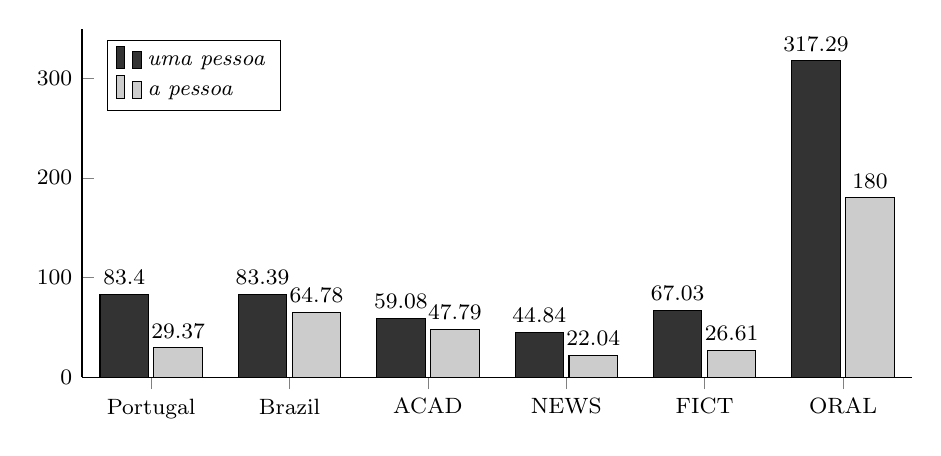
\begin{tikzpicture}
      \begin{axis}
		  [ybar,
		   ymin=0,
		   font={\footnotesize},
		   bar width=1.75em,
		   xtick=data,
		   axis lines*=left,
		   symbolic x coords={Portugal,Brazil,ACAD,NEWS,FICT,ORAL},
		   nodes near coords,
		   width=\textwidth,
		   height=6cm,
		   legend pos=north west,
		   legend cell align=left
		  ]
		  \addplot+ [black,fill=black!80] coordinates {(Portugal, 83.4)
		  	(Brazil,    83.39)
		  	(ACAD,      59.08)
		  	(NEWS,      44.84)
		  	(FICT,      67.03)
		  	(ORAL,      317.29)
		  };
		  \addlegendentry{\textit{uma pessoa}}
		  \addplot+ [black,fill=black!20] coordinates
		  {(Portugal,  29.37)
		  	(Brazil,    64.78)
		  	(ACAD,      47.79)
		  	(NEWS,      22.04)
		  	(FICT,      26.61)
		  	(ORAL,      180)
		  };
	  	  \addlegendentry{\textit{a pessoa}}
		\end{axis}
  \end{tikzpicture}
  \caption{\label{fig:amaral:1}Frequencies of the expressions \textit{a pessoa}/\textit{uma pessoa} in the 20th century, CDP (per million words) in EP and BP and different genres.}
\end{figure}



Although the data come from different sources (most importantly, we do not have oral data from prior to the 1970s), the data might reflect an increase from the 19th to the 20th century. Alternatively, the increase in impersonal uses starts earlier, but this is not evident in the available written data. Interestingly, in the 19\textsuperscript{th} {century} {\textit{uma pessoa}} {prevails both in EP and BP. In both subcorpora in NURC} {\textit{a pessoa} }{clearly prevails, a comparison of the subcorpus from the 1970s and 1990s shows that the proportion of} {\textit{uma pessoa}} {diminishes}, as shown in \figref{fig:amaral:2}.




\begin{figure}
    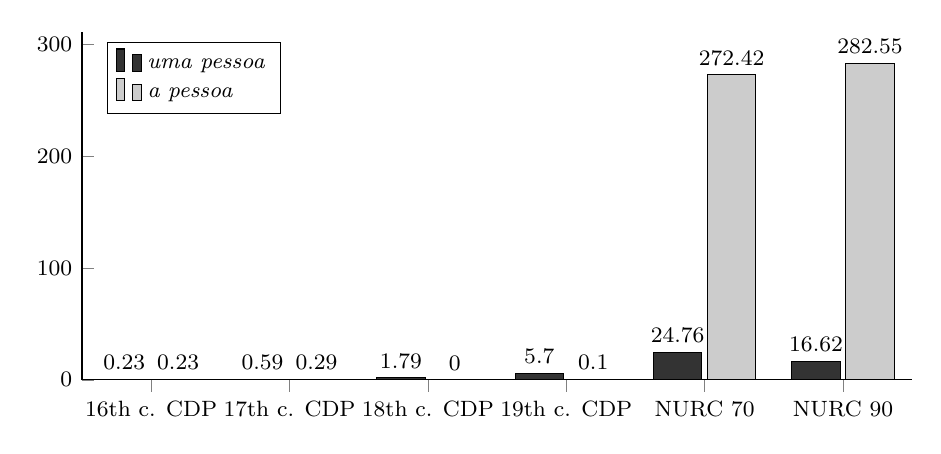
\begin{tikzpicture}
        \begin{axis}
		  [ybar,
           ymin=0,
		   font={\footnotesize},
		   bar width=1.75em,
		   xtick=data,
		   axis lines*=left,
		   symbolic x coords={16th c. CDP,17th c. CDP,18th c. CDP,19th c. CDP,NURC 70,NURC 90},
		   nodes near coords,
		   width=\textwidth,
		   height=6cm,
		   legend pos=north west,
		   legend cell align=left
		  ]
		  \addplot+ [black,fill=black!80] coordinates {(16th c. CDP,0.23)
		  	(17th c. CDP,0.59)
		  	(18th c. CDP,1.79)
		  	(19th c. CDP,5.7)
		  	(NURC 70,24.76)
		  	(NURC 90,16.62)
		  };
		  \addlegendentry{\textit{uma pessoa}}
		  \addplot+ [black,fill=black!20] coordinates
		  {(16th c. CDP,0.23)
		  	(17th c. CDP,0.29)
		  	(18th c. CDP,0)
		  	(19th c. CDP,0.1)
		  	(NURC 70,272.42)
		  	(NURC 90,282.55)
		  };
	  	  \addlegendentry{\textit{a pessoa}}
		\end{axis}
    \end{tikzpicture}
    \caption{\label{fig:amaral:2}Impersonal \textit{a pessoa} and \textit{uma pessoa} in CDP and NURC RJ for the ’70s and ’90s (in subject position, per million words).}
\end{figure}



\subsection{Contemporary oral data from Rio de Janeiro and Minas Gerais}\label{sec:amaral:5.3}

The comparison of the oral data from the 1970s, 1990s, 2010s and 2020s show that the proportion between {\textit{uma pessoa}} {and} {\textit{a pessoa}} {– with impersonal} {\textit{a pessoa}} {being far more frequent than} {\textit{uma pessoa}} – remains relatively stable, with a slight increase of {\textit{uma pessoa}} {from the 1990s to the 21st century, and a more pronounced growth in the use of}{ \textit{a pessoa}} {in the 21st}{\textsuperscript{} }{century in comparison with the 20th. The comparison of} {\textit{a pessoa}} {and} {\textit{uma pessoa}} {in the samples from the 2010s and 2020s does not show great differences (this is also true for the referential types and contexts, discussed in \sectref{sec:amaral:6}). The analyses of the frequency of} {\textit{a pessoa}} {and} {\textit{uma pessoa}} {in two contemporary samples of BP also offer important insights in terms of regional variation. There are no significant differences between the 21st{}-century data from CORPORAPORT Rio de Janeiro and Minas Gerais MOC (see \figref{fig:amaral:3}). Considering previous studies of} {\textit{a pessoa}} {and} {\textit{uma pessoa}} {in BP and EP, the results allow us to suppose that perhaps more significant differences can be found between BP and EP than between different Brazilian dialects.} 


\begin{figure}
    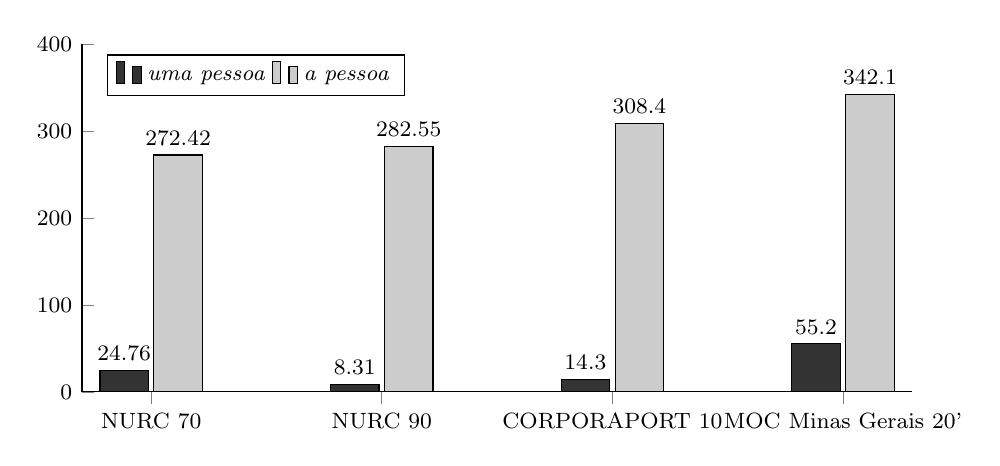
\begin{tikzpicture}
        \begin{axis}
		  [ybar,
           ymin=0,
           ymax=400,
		   font={\footnotesize},
		   bar width=1.75em,
		   xtick=data,
		   axis lines*=left,
		   symbolic x coords={NURC 70,NURC 90,CORPORAPORT 10,MOC Minas Gerais 20'},
		   nodes near coords,
		   width=\textwidth,
		   height=6cm,
		   legend pos=north west,
		   legend columns=-1,
		   legend cell align=left,
		  ]
		  \addplot+ [black,fill=black!80] coordinates {(NURC 70,24.76)
		  	(NURC 90,8.31)
		  	(CORPORAPORT 10,14.3)
		  	(MOC Minas Gerais 20',55.2)
		  };
		  \addlegendentry{\textit{uma pessoa}}
		  \addplot+ [black,fill=black!20] coordinates
		  {(NURC 70,272.42)
		  	(NURC 90,282.55)
		  	(CORPORAPORT 10,308.4)
		  	(MOC Minas Gerais 20',342.1)
		  };
	  	  \addlegendentry{\textit{a pessoa}}
		\end{axis}
    \end{tikzpicture}
    \caption{\label{fig:amaral:3}20th- and 21st-century oral data (impersonal uses in subject position per million words)}
\end{figure}



The following examples illustrate contemporary uses. In example \REF{ex:amaral:31}, the participant comments on the current facilities for students. In this context, he uses {\textit{a pessoa}} {to express the general statement that if one wants to study it is easy because there are many possibilities. Note that after using the formally feminine NP} {\textit{a pessoa}}{, the participant anaphorically refers back with the masculine personal pronoun} {\textit{ele} }{‘he’. \citet[13]{Posio2021} mentions the same phenomenon when he analyses occurrences of} {\textit{uma pessoa}}{. The author has no explanation for the observation that masculine agreement is found only with indefinite form} {\textit{uma pessoa}} {but not with the definite} {\textit{a pessoa}} {in the corpus of EP he mentions. Masculine agreement is also common with the grammaticalised pronoun} {\textit{a gente}}{, which also goes back to a feminine noun, and it is unsurprising that the same kind of agreement can be observed in} {\textit{pessoa} }{constructions. Both} {\textit{gente}} {(‘people’) and} {\textit{pessoa}} {(‘person’) are feminine nouns in their original lexical meaning, and the masculine anaphors therefore point to a loss of the feminine gender in the process of pronominalisation (see \citealt{Lopes2004} on the changes in agreement of} {\textit{a gente}} {in the course of grammaticalisation).}\largerpage[-1]



\eanoraggedright\label{ex:amaral:31}
porque eu trabalho e estudo né eu faço os dois eu não deixei de trabalhar pra poder estudar pros concursos... isso acaba apertando o horário você tem que estudar até mais tarde final de semana você acaba estuDANdo ...\\
{[...]}\\
{[...]} hoje em dia tem tanto curso tem tanta:: tanta facilidade de acesso à informaÇÃO:: à/ à AUla te/ tem aula telepresenciAL tem: um monte de facilidade ... [...] eu acho que se \ExHighlight{a pessoa} quiser estudar mesmo pode ser o que FOR \ExHighlight{ele} vai assim você hoje tem MUIto CURso eh:... (COP-A-3-M, male, 31 years old, high educational level)\pagebreak
\glt ‘because I work and study, you know? I do both I didn’t stop working to study for the public contests... this ends up tightening the schedule you have to study late on weekends you end up studying... [...]\\
{[...] nowadays there are so many courses there is so much:: it’s so easy to have access to information:: to/ to the CLASS you/ there are non presential classes there is: everything is so easy... [...] I think if \ExHighlight{the person} really wants to study anything} \ExHighlight{he} {will, so today you have a LOT of COURSES eh:...’}
\z 


{Examples with a similar interpretation to the ones above appear in the recent data collected in Minas Gerais. In example \REF{ex:amaral:32}, the interviewer and the participant talk about physical exercise. The participant admits that he does not do any sports, but after that states that it is important for health. To justify that statement, he uses the generalising NP} {\textit{a pessoa}}. 



\eanoraggedright\label{ex:amaral:32}
{Interviewer:} {{...tem algum outro esporte de que o sinhô gosta?}}\\
{Participant:} {{uah tem esporte que eu gosto só que eu num eu praticamente num tô pratican[d]o quase nenhum caminhada né éh fazer caminhada exercício físico isso é muito bom é necessário}} \ExHighlight{a pessoa} fazer para a saúde {(MOC 19 - J.F, male, 59 years old, low educational level)}
\glt 
`{Interviewer:} {...is there any other sport you like?}
{Participant:} why, there are sports that I like but I don’t practise any like walking, you know, walking physical exercise that’s very good it’s necessary for {\ExHighlight{the person/one}} {to do it for one’s health’}
\z 


In example \REF{ex:amaral:33}, the inclusion of speaker and addressee can also be observed. The interviewer uses the first person pronoun {\textit{nós}} {and the participant answers with the NP} \textit{a pessoa}. Both uses are close to the universal generic function 5 in \tabref{tab:amaral:1}.



\eanoraggedright\label{ex:amaral:33}
{Interviewer:} {ok intão em sua opinião qual é o nosso destino depois da morte? pra onde nós vamos?}\\
{Participant:} depois da morte \ExHighlight{a pessoa} vai ter um lugar de repouso né de descanso né com Deus é a promessa da palavra de Deus após a morte \ExHighlight{a pessoa} terá ôta vida cum Deus né (MOC 19 - J.F, male, 59 years old, low educational level)
\glt `{Interviewer:} ok so in your opinion what is our fate after death? where are we going to?\\
      Participant: {after death} \ExHighlight{we/one} will have a place to rest, you know, rest with God, it’s the promise of the word of God after death \ExHighlight{we/one} will have great life with God, you know’
\z 


{According to our own observations in informal speech conducted in Brazilian Portuguese,}\footnote{{The corpora mentioned in \figref{fig:amaral:3} include sociolinguistic interviews and are therefore less colloquial than, say, free conversations or occurrences derived from the internet.}} {especially with younger speakers,} {\textit{a pessoa aqui}} {acquires an interpretation equivalent to the first person pronoun}{. }{In all the examples below, written in informal blogs and found through a search in} {\textit{Corpus do Português – Web/dialects}}{, the speaker uses this construction as a first person pronoun:} 


\eanoraggedright\label{ex:amaral:34}
Ana, querida, ainda não postei seus selinhos, a homenagem e o prêmio dardos, mas é que {\ExHighlight{a pessoa aqui}} tá mesmo enrolada tá? Não é falta de atenção e carinho nao, tá? (\url{http://anamgs.blogspot.com/2010/06/gente-se-acostuma.html})
\glt ‘Ana, dear, I haven’t posted your stamps, the homage and the Dardos award yet, but {\ExHighlight{the person here}} {(=} {\ExHighlight{I)}} {is really messed up, right? It’s not a lack of attention and affection, right?’}
\ex\label{ex:amaral:35}No box tinha uma cortina, bem fofa, porque \ExHighlight{a pessoa aqui} sempre gostou de coisas fofas né? (\url{http://cassisfamilia.blogspot.com/2013/06/minha-casa-linda-e-com-meu-jeito-meu.html}) 
\glt ‘In the bathroom stall there was a curtain, very cute, because \ExHighlight{the person here} (= \ExHighlight{I}) always liked cute things, right?’
\z 


This might point to a use in the direction of a first person pronoun, thus suggesting an interpretation similar to \textit{a gente} (for instance \citealt{Lopes2004}) and French \textit{on} (see \citealt{Coveney2000}).


The cases with \textit{uma pessoa} are less frequent, though it is worth citing some examples. In example \REF{ex:amaral:36}, there is an exclusive interpretation. In example \REF{ex:amaral:37}, the participant uses the NP \textit{uma pessoa} and also \textit{a pessoa} (possibly anaphorically referring to the impersonal antecedent \textit{uma pessoa})  in a sequence of conditional clauses. Note that these are cases close to the lexical use with a first indefinite NP and a following anaphoric NP: 

\eanoraggedright\label{ex:amaral:36}
não acredito que \ExHighlight{uma pessoa} se sinta plena ou realizada vivendo de esmola vivendo de migalhas eu acho que se e/ \ExHighlight{elas} deveria(m) ter a oportunidade de ser cidadões cidadãos né tudo (COP-A-2-M, male, 19 years old, middle educational level)
\glt ‘I don't believe that \ExHighlight{a person/one} {feels full or fulfilled, living on alms, living on crumbs I think if and/}{\ExHighlight{they}} should have the opportunity to be citizens, you know?’
\ex\label{ex:amaral:37}com a reforma mudou muito isso mais se num tiver emprego num tem comida num tem como \ExHighlight{uma pessoa} pagar uma água num tem como \ExHighlight{a pessoa}  pagar uma luz aí cumeça num estado que \ExHighlight{a pessoa} ou então mesmo a comprar \ExHighlight{a pessoa} as vez prefere comprar comida dentro de casa do que comprar uma roupa {(MOC 07 - A.R, male, 25 years old, high educational level)}
\glt ‘with the reform this has changed a lot, but if you don’t have a job, you don’t have food, \ExHighlight{the person/one} doesn’t have money to pay for water there is no way to pay for electricity, then it reaches a state that you are even buying, you sometimes prefers to buy food at home than buy clothes’
\z 


\section{Diachronic and diatopic tendencies of functional differentiation}\label{sec:amaral:6}



The general impression from existing studies on BP (\citealt{AmaralMihatsch2019}) and EP (\citealt{Posio2021}, \citealt{Martins2022}) is that \textit{a pessoa} {and} \textit{uma pessoa} specialise in non-episodic uses, i.e. functions 5 to 7 in \tabref{tab:amaral:1}. They also agree on the essentially inclusive or speaker-oriented character and their tendency to occur in generalisation strategies.



We analysed the corpora across the centuries according to the functions in \tabref{tab:amaral:1}, isolated uses in inclusive as well as exclusive contexts. \figref{fig:amaral:4} illustrates percentages of the respective impersonal uses; as explained above, CORPORAPORT contains data from the 2010s and MOC from 2020.

\vfill
\begin{figure}[H]
	\pgfplotsset{cycle list/PuOr-4}
	\begin{tikzpicture}
		\begin{axis}
			[ybar,
			ymin=0,
			ymax=90,
			x=1.99cm,
			bar width=8pt,
			font={\footnotesize},
			xtick=data,
			axis lines*=left,
			symbolic x coords={16–18th c. CDP,19th c. CDP,NURC 70,NURC 90,CORPORAPORT,MOC},
			nodes near coords,
			nodes near coords style={rotate=90, anchor=west},
			width=\textwidth,
			height=6cm,
			legend columns=-1,
			legend pos=north west,
			legend cell align=left,
			cycle list name=PuOr-4,
			every axis plot/.append style={fill}
			]
			\addplot coordinates {(16–18th c. CDP,0)
				(19th c. CDP,0.2)
				(NURC 70,0)
				(NURC 90,2.8)
				(CORPORAPORT,0)
				(MOC,9.7)
			};
			\addlegendentry{Functions 1–3}
			\addplot coordinates
			{(16–18th c. CDP,30)  
				(19th c. CDP,8.6)
				(NURC 70,45.8)
				(NURC 90,41.7)
				(CORPORAPORT,60)
				(MOC,47.2)
			};
			\addlegendentry{Function 4}
			\addplot coordinates
			{(16–18th c. CDP,50)
				(19th c. CDP,     31)
				(NURC 70,         12.5)
				(NURC 90,         8.3)
				(CORPORAPORT,     13)
				(MOC,             22.2)
			};
			\addlegendentry{Function 5}
			\addplot coordinates
			{(16–18th c. CDP,20)
				(19th c. CDP,     58.7)
				(NURC 70,         41.7)
				(NURC 90,         47.2)
				(CORPORAPORT,     26.7)
				(MOC,             20.8)
			};
			\addlegendentry{Functions 6–7}
		\end{axis}
	\end{tikzpicture}
	\caption{\label{fig:amaral:4}The functional development of \textit{a pessoa} and \textit{uma pessoa} (\% of uses) in diachrony in subject position}
\end{figure}
\vfill\pagebreak


Functions 4, 5, 6 and 7 (the latter two taken together) appear from the first attestations on, although sporadically. The most frequent non-veridical (mainly hypothetical) uses in the 19\textsuperscript{th} century (functions 6 and 7) decrease in proportion in the 20th and 21st century, the generalising function 4 comes to prevail from the second half of the 20th century and episodic uses first appear in the 19th century and show a slight increase in the contemporary data. This picture shows an increasing functional diversification in the course of grammaticalisation. It is hard to pin down one of the functions as a starting point of the emergence of the impersonal function. General statements and universal truths prevail in the isolated uses before the 19th century, while in the 19th century non-veridical uses dominate. These overlap with function 7, which also links indefinite (non-impersonal) uses and impersonal interpretations, since conditionals tend to allow both interpretations (see \sectref{sec:amaral:3}). Possibly these contexts contributed to an entrenchment of the impersonal function.



Although episodic uses are rare, they have been attested (see \citealt{AmaralMihatsch2019}). Our observations, as well as those of \citet{Posio2021}, suggest a transitional context and degrees of episodicity, with narratives in the past (especially what \citet{KitagawaLehrer1990} call “life drama” narrations) occupying an intermediate position between generic and episodic uses. The distance from the moment of speaking possibly leads to a greater degree of vagueness and lesser specificity of episodic impersonals in the past in comparison to uses in the present. The following examples may illustrate this transition zone. In \REF{ex:amaral:38} the informant answers the interviewer’s question regarding whether the informant has experienced a potentially lethal situation before, although the use of negation gives this episodic use a hypothetical flavor:\largerpage



\ea\label{ex:amaral:38} 
{Interviewer:} {{intendi... tirando isso você nunca passou por nenhum outro problema não?}}\\
{Participant:} {{não}}\\
{Interviewer:} {{você já presenciou algum acidente?}}\\
{Participant:} de moto assim na / nada grave nada que \ExHighlight{a pessoa} saiu de lá muito grave nada não acidente comum de / de esquina esses trem assim
(MOC 13 - A.J, female, 37 years old, low educational level)
\glt
`{Interviewer:} {I see... other than that, you never had any other problems did you?}\\
{Participant:} {no}\\
{Interviewer}{: Have you ever witnessed an accident?}\\
{Participant}{: on a motorcycle like that in / nothing serious, nothing that} {\ExHighlight{the} \ExHighlight{person/one}} {came out seriously injured, nothing not, common accident on / around corners and things like that’}
\z 


In \REF{ex:amaral:39}  \textit{a pessoa} refers to the speaker’s mother in a specific situation, but one might think alternatively about a general statement about the length of the trip at that time, so here, the episodic character is not entirely clear either, although the perfect rather suggests an episodic use (interestingly \textit{uma pessoa} {precedes} \textit{a pessoa}):



\eanoraggedright\label{ex:amaral:39}
meu avô... ele... foi... destacado pro sul... e a minha mãe não podia ir porque ia formar... ia acabar... o... o normal... então ficou pra depois encontrar com eles... eles foram pra depois ela ir... QUANdo a minha mãe foi... eh... não tinha aquela... aquela... ( ) tem hoje né... era um navio bem... bem fulerazinho... fulerazinho... então... coitadinha ela foi... sozinha... foi embora pro sul... e pegou uma tempestade em alto mar... diz ela que a água passava... então ela tinha verdadeiro pavor... não é pra menos... eu acho que \ExHighlight{uma pessoa} ... já pensou? à noite... \ExHighlight{a pessoa} levou muito tempo pra chegar no sul né... pegou essa tempestade em pleno... alto mar... {(NURC 90 complementar)}
\glt ‘my grandfather... he... was... transferred to the south... and my mother couldn’t go because she finished her studies... she finished... the... normal course... then she agreed to meet them later... they went so that she should go later... WHEN my mother went... eh... there wasn’t that one... that one... ( ) there is today, right... it was a ship quite...quite tiny... tiny... so... she went... alone... she went to the south... and caught a storm on the high seas... she says the water passed... so she was really terrified... no wonder... I think \ExHighlight{a person/one} ... have you thought about it? at night... \ExHighlight{the person/one} took a long time to reach the south, right... she caught this storm... on the high sea...’
\z 


The inclusive quasi-episodic uses do not fit into Gast \& van der Auwera’s characterisation of exclusive episodic uses – here, rather than showing a development towards a use as a first person pronoun, we think the type of pronominalisation source, linked to inclusive uses in generalising statements, seems to affect the exact sequence of emerging new functions and functional expansion. This is a case of persistence in the course of grammaticalisation following \citet{Hopper1991}. However, we cannot exclude an evolution of episodic inclusive uses taking over the function of first person pronouns as in \REF{ex:amaral:34} which, according to our research, is possibly more frequent in young people’s speech nowadays. Unfortunately the Web/dialects corpus does not give us the age of the writers. 

\figref{fig:amaral:5} highlights the frequencies of inclusive and exclusive uses.{\interfootnotelinepenalty=10000\footnote{As pointed out above, the CDP data are based on written texts, while NURC, CORPORAPORT and MOC are oral corpora. Thus a comparison of the data up to the 19th century and the 20th and 21st century has to be interpreted with great caution.}} The proportion of uses in inclusive contexts decreases over time. Inclusive or speaker-oriented uses characterise the earlier uses leading to the evolution of these impersonals while exclusive uses arise later and tend to increase until the 2010s data, with a slight decrease in 2020. 

\pgfplotsset{cycle list/PuOr-4}
\begin{figure}
    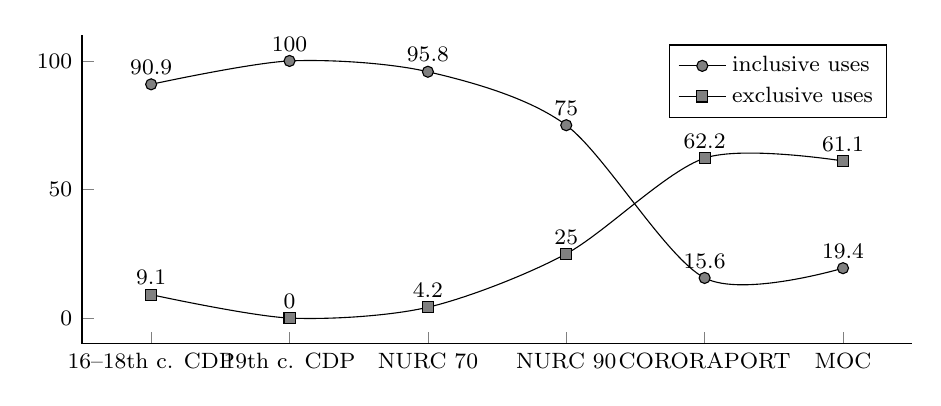
\begin{tikzpicture}
        \begin{axis}
		  [smooth,
		   font={\footnotesize},
		   xtick=data,
		   axis lines*=left,
		   symbolic x coords={16–18th c. CDP,19th c. CDP,NURC 70,NURC 90,CORORAPORT,MOC},
		   nodes near coords,
		   width=\textwidth,
		   height=5.5cm,
		   legend pos=north east,
		   legend cell align=left,
		   cycle list name=black white
		  ]
		  \addplot+ coordinates {(16–18th c. CDP,90.9)
		  	(19th c. CDP,100)
		  	(NURC 70,95.8)
		  	(NURC 90,75)
		  	(CORORAPORT,15.6)
		  	(MOC,19.4)
		  };
		  \addlegendentry{inclusive uses}
		  \addplot+ coordinates
		  {(16–18th c. CDP,9.1)
		  	(19th c. CDP,0)
		  	(NURC 70,4.2)
		  	(NURC 90,25)
		  	(CORORAPORT,62.2)
		  	(MOC,61.1)
		  };
	  	  \addlegendentry{exclusive uses}
		\end{axis}
    \end{tikzpicture}
    \caption{\label{fig:amaral:5}The functional development of \textit{a pessoa} and \textit{uma pessoa} (\% of uses in the respective corpus) taken together in diachrony in subject position.}
\end{figure}


The reversal of frequency of \textit{uma pessoa} to \textit{a pessoa} in the 20th century in BP (see \figref{fig:amaral:2}) differs from the observations for EP in \citet{Posio2021} and \citet{Martins2022} as well as in \citet[147]{Afonso2008} who argue in favour of a higher frequency of \textit{uma pessoa} in EP. The fact that the impersonal expression {\textit{a pessoa}} {is more frequent might be a result, at least for Brazilian Portuguese, of the greater frequency of anaphoric NPs in longer chains of reference as opposed to the originally indefinite} {\textit{uma pessoa}}. 


We have postulated above that \textit{a pessoa} {and} \textit{uma pessoa} follow the same grammaticalisation path, so we would then also expect comparable functional profiles. Since \textit{uma pessoa} is very infrequent in our corpus data, we conducted a survey based on acceptability judgments (see \sectref{sec:amaral:4} on the survey design). We used a Likert scale from 1 (perfectly acceptable) to 5 (unacceptable) und tested equivalents of the diagnostic sentences of \citet{GastvanderAuwera2013} and additional sentences for each function (see \figref{fig:amaral:6}).\largerpage[1.75]


\begin{figure}
    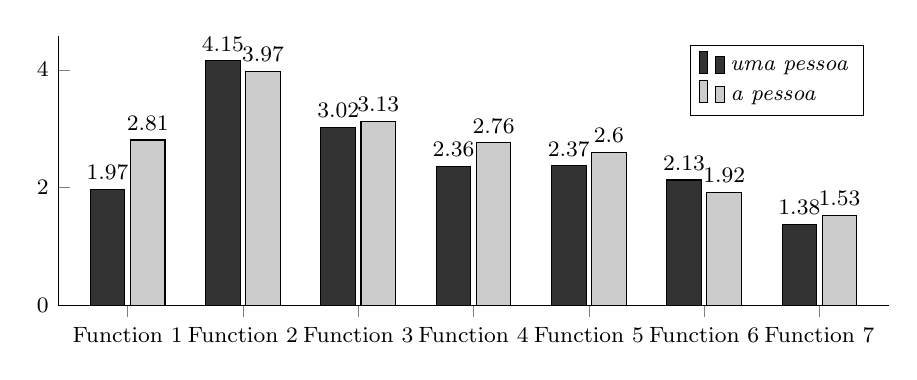
\begin{tikzpicture}
        \begin{axis}
		  [ybar,
		   ymin=0,
		   font={\footnotesize},
		   bar width=1.25em,
		   xtick=data,
		   axis lines*=left,
		   symbolic x coords={Function 1,Function 2,Function 3,Function 4,Function 5,Function 6,Function 7},
		   nodes near coords,
		   width=\textwidth,
		   height=5cm,
		   legend pos=north east,
		   legend cell align=left
		  ]
		  \addplot+ [black,fill=black!80] coordinates {(Function 1,1.97)
		  	(Function 2,4.15)
		  	(Function 3,3.02)
		  	(Function 4,2.36)
		  	(Function 5,2.37)
		  	(Function 6,2.13)
		  	(Function 7,1.38)
		  };
		  \addlegendentry{\textit{uma pessoa}}
		  \addplot+ [black,fill=black!20] coordinates
		  {(Function 1,2.81)
		  	(Function 2,3.97)
		  	(Function 3,3.13)
		  	(Function 4,2.76)
		  	(Function 5,2.6)
		  	(Function 6,1.92)
		  	(Function 7,1.53)
		  };
	  	  \addlegendentry{\textit{a pessoa}}
		\end{axis}
    \end{tikzpicture}
    \caption{\label{fig:amaral:6}Degrees of acceptabilty of \textit{a pessoa} and \textit{uma pessoa} in diagnostic functions (high values indicate lower acceptability).}
\end{figure}


{We tested the statistical significance of the differences between the acceptability of the two expressions for each function and only found a significant difference for function 1 (applying the Games-Howell post hoc test}\footnote{Only for condition 1 was \textit{a pessoa} rated significantly higher than \textit{uma pessoa} ($p < 0.001$). See Appendix~\ref{appendix:amaral} for test results.}). 
% % % For \textit{a pessoa}, we obtained the following results when applying the Games-Howell post hoc test: 
% % % condition 8 was rated significantly higher than cond. 1 (p = .000), 3 (p = .001), 4 (p = .000), 5 (p = .000), 6 (p = .000), 7 (p = .000), 9 (p = .000), 10 (p = .000) and 11 (p = .028).
% % % condition 2 was rated significantly higher than cond. 1 (p = .000), 4 (p = .000), 5 (p = .002), 6 (p = .000), 7 (p = .000), 9 (p = .000) und 10 (p = .005).
% % % condition 6 was rated significantly higher than cond. 1 (p = .000), 2 (p = .000), 3 (p = .000), 4 (p = .004), 8 (p = .000), 10 (p = .005) and 11 (p = .003).
% % % condition 7 was rated significantly lower than cond. 1 (p = .000), 2 (p = .000), 3 (p = .000), 4 (p = .000), 5 (p = .017), 8 (p = .000), 9 (p = .000), 10 (p = .000) and 11 (p = .000).
% % % {For} {\textit{uma pessoa}} {we obtained the following results:}
% % % condition 2 was rated significantly higher than cond. 1 (p = .000), 3 (p = .000), 4 (p = .000), 5 (p = .000), 6 (p = .000), 7 (p = .000), 10 (p = .000) and 11 (p = .000).
% % % condition 8 was rated significantly higher than cond. 1 (p = .000), 4 (p = .000), 5 (p = .001), 6 (p = .000), 7 (p = .000), 10 (p = .022) und 11 (p = .000).
% % % condition 3 was rated significantly higher than cond. 1 (p = .000), 6 (p = .008), 7 (p = .000) and 11 (p = .000); but signif. lower than cond. 2 (p = .000).
% % % condition 10 was rated significantly higher than cond. 1 (p = .001), 6 (p = .042), 7 (p = .000) and 11 (p = .002); but signif. lower than cond. 2 (p = .000) and 8 (p = .022).
% % % condition 7 was rated significantly lower than cond. 1 (p = .018), 2 (p = .000), 3 (p = .000), 4 (p = .000), 5 (p = .036), 6 (p = .007), 8 (p = .000) und 10 (p = .000).
Function 1 also allows an indefinite interpretation of \textit{uma pessoa}, so the participants probably did not judge the impersonal use, despite the instruction to consider only impersonal interpretations. The near identity of both forms in all other cases is a striking confirmation of the functional equivalence in BP. The data also show an increasing acceptability from function 2 to function 7, which backs our corpus analysis, i.e. the preference for non-episodic inclusive uses. The position of function 1 is harder to explain. It is possible that the informants interpreted the sentences as having a personal/referential interpretation.



Finally, when discussing the evidence of the grammaticalisation of \textit{a/uma pessoa}, \citet[12]{Posio2021} mentions the issue of the repetition of the noun phrase to refer to itself, instead of using a personal pronoun. The author comments that in his data there are no cases where the personal pronoun \textit{ela} ‘she’ is used to refer back to the NP. Contrary to what the author observes for EP, our data present occurrences with this context \REF{ex:amaral:40}, as well as occurrences where the whole NP is repeated \REF{ex:amaral:41}. However, unlike what the author finds for EP, according to the first author of this paper \textit{uma pessoa} does not allow this kind of repetition in BP (although we detected one example in C-ORAL-Brasil, see \citealt{AmaralMihatsch2019}). Therefore, an example like \REF{ex:amaral:41} seems to be unacceptable in BP, while \REF{ex:amaral:40} is acceptable. The samples thus corroborate the existence of differences between the two varieties of Portuguese, especially when analysing the frequency and the paths of grammaticalisation of \textit{uma pessoa}.



\eanoraggedright\label{ex:amaral:40}
% % ... o povo hoje tá mais assim atento né aos seus direitos \ExHighlight{a pessoa} corre atrás mermo porque \ExHighlight{a pessoa} sabe dos seus direito aquilo que \ExHighlight{ele} num sabe ele busca informação (MOC 19 - J.F, male, 59 years old, low educational level)
% % \glt ‘... the people today are more aware of their rights, the person runs after it because the person knows their rights, what they don’t know they seek information’
às vezes \ExHighlight {a pessoa} ela gosta de assistir um jornal e ela não tem... é custume de assistir um otro... \citep{Amaral2015}
\glt `sometimes \ExHighlight{one} (lit. 'the person', feminine)  she likes to watch a news programme and she is not used to watch another one.'
\ex\label{ex:amaral:41} 
Mas esse peixe, já \ExHighlight{uma pessoa} às vezes não o conhece. Não sabe de que peixe é, não é? Se \ExHighlight{uma pessoa} visse a figura do peixe, já \ExHighlight{uma pessoa} dizia: “Olha, pode ser a sardinha, pode ser carapau”. (CORDIAL-SIN, VPA-30)
\glt ‘But that fish, sometimes \ExHighlight{a person} does not even recognise it. They don’t know what fish it is, right? If \ExHighlight{a person} saw the form of the fish, \ExHighlight{a person} would say: “Look, it can be a sardine, it can be a mackerel.”’ \citep[13]{Posio2021}
\z 

\section{Conclusion}\label{sec:amaral:7}

In this paper we discussed the functions of inclusive impersonal uses of \textit{a pessoa} and \textit{uma pessoa} in Brazilian Portuguese in order to shed light on the diachronic development of the restrictions determining impersonal uses and the differences and parallels between the two expressions.


First, it should be highlighted that the development of impersonal uses detectable in our data – as well as their synchronic properties – point to parallels in the origins of \textit{a pessoa} {and} \textit{uma pessoa}, although the grammaticalisation process then leads to a subsequent, mainly diatopical differentiation. In our Brazilian oral data \textit{a pessoa} very clearly prevails. Their impersonal function becomes evident when trying to translate the impersonal attestations into other languages that have nouns derived from Latin \textit{persona} such as Spanish \textit{persona}, French  \textit{personne} {or English} {\textit{person.}} {The translation requires an impersonal pronoun such as English} {\textit{one}} {or French} {\textit{on}}. 



{The first impersonal occurrences in the 16th and 17th centuries are scarce. The situation changes in the 19th century, when there is an increase, especially in the incidence of} {\textit{uma pessoa}}{. In the second half of the 20th century Brazilian Portuguese, however, clearly prefers the impersonal} {\textit{a pessoa}}{, although} {\textit{uma pessoa}} is also used. A classification of the occurrences from two different varieties of BP showed a similar pattern of behaviour of the two expressions.



{From  the 16}{\textsuperscript{th}} {century to the 21}{\textsuperscript{st}} {century they have shown a clear preference for inclusive, non-episodic uses up to the 21}{\textsuperscript{st}} {century, although our corpus data threw up results that reveal a functional shift and a certain functional expansion, notably exclusive and epidsodic uses, in the course of grammaticalisation of the two expressions. Some occurrences even show a tendency toward first person pronoun uses, so it is certainly worth continuing this research with recent data from young speakers.}


\appendixsection{Games-Howell post hoc test results}\label{appendix:amaral}

\begin{table}[H]\small
\caption{\label{tab:amaral:a1}Games-Howell post hoc test results. “H” rating indicates higher rating, “L” lower.}
		\begin{tabular}{ *2{lcS[table-format=<1.3]} }
			\lsptoprule
			\multicolumn{3}{c}{\textit{a pessoa}} & \multicolumn{3}{c}{\textit{uma pessoa}}\\\cmidrule(lr){1-3}\cmidrule(lr){4-6}
			Comparison & Rating & {$p$} & Comparison & Rating & {$p$}\\\midrule
			8:1   & H & <0.001     &  2:1   & H & <0.001\\
			8:3   & H & 0.001      &  2:3   & H & <0.001\\
  			8:4   & H & <0.001     &  2:4   & H & <0.001\\
  			8:5   & H & <0.001     &  2:5   & H & <0.001\\
  			8:6   & H & <0.001     &  2:6  & H & <0.001\\
  			8:7   & H & <0.001     &  2:7  & H & <0.001\\
  			8:9   & H & <0.001     &  2:10   & H & <0.001\\
  			8:10  & H & <0.001     &  2:11   & H & <0.001\\
			8:11  & H & 0.028      &   8:1   & H & <0.001\\
			2:1   & H & <0.001     &  8:4   & H & <0.001\\
			2:4   & H & <0.001     &  8:5   & H & 0.001\\
			2:5   & H & 0.002      &   8:6  & H & <0.001\\
			2:6   & H & <0.001     &  8:7  & H & <0.001\\
			2:7   & H & <0.001     &  8:10   & H & 0.022\\
			2:9   & H & <0.001     &  8:11   & H & <0.001\\
			2:10   & H & 0.005     &  3:1   & H & 0.001\\
			6:1   & H & <0.001     &  3:2   & L & <0.001\\
			6:2   & H & <0.001     &  3:6  & H & 0.008\\
			6:3   & H & <0.001     &  3:7  & H & <0.001\\
			6:4   & H & 0.004      &   3:11   & H & <0.001\\
			6:8   & H & <0.001     &  10:1   & H & 0.001\\
			6:10   & H & 0.005     &  10:2   & L & <0.001\\
			6:11   & H & 0.003     &  10:6  & H & 0.042\\
			7:1   & L & <0.001     &  10:7  & H & <0.001\\
			7:2   & L & <0.001     &  10:8  & L & 0.022\\
			7:3   & L & <0.001     &  10:11   & H & 0.002\\
			7:4   & L & <0.001     &  7:1   & L & 0.018\\
			7:5   & L & 0.017      &   7:2   & L & <0.001\\
			7:8   & L & <0.001     &  7:3   & L & <0.001\\
			7:9   & L & <0.001     &  7:4   & L & <0.001\\
			7:10   & L & <0.001    & 7:5   & L & 0.036\\
			7:11   & L & <0.001    & 7:6   & L & 0.007\\
			       &   &           &   7:8   & L & <0.001\\
			       &   &           &   7:10  & L & <0.001\\
			\lspbottomrule
		\end{tabular}
\end{table}

\section*{Acknowledgements}


We would like to thank two anonymous reviewers for their valuable suggestions, Désirée Kleineberg for her help with the statistical analysis of the judgment data, Welber Nobre dos Santos for the data collection for the MOC corpus and Ina Berner for helping to prepare the NURC data for analysis.

\printbibliography[heading=subbibliography]
\end{document}
